%% 
%% Copyright 2019-2020 Elsevier Ltd
%% 
%% This file is part of the 'CAS Bundle'.
%% --------------------------------------
%% 
%% It may be distributed under the conditions of the LaTeX Project Public
%% License, either version 1.2 of this license or (at your option) any
%% later version.  The latest version of this license is in
%%    http://www.latex-project.org/lppl.txt
%% and version 1.2 or later is part of all distributions of LaTeX
%% version 1999/12/01 or later.
%% 
%% The list of all files belonging to the 'CAS Bundle' is
%% given in the file `manifest.txt'.
%% 
%% Template article for cas-dc documentclass for 
%% double column output.

%\documentclass[a4paper,fleqn,longmktitle]{cas-dc}
% \documentclass[a4paper,fleqn]{cas-dc}
\documentclass{singlecol-new}

%\usepackage[authoryear,longnamesfirst]{natbib}
%\usepackage[authoryear]{natbib}
\usepackage[numbers]{natbib}

\usepackage{amsmath,amssymb}
\usepackage{longtable}
%%%
\usepackage{mathtools}
\allowdisplaybreaks
\usepackage{algorithm,algorithmic}
\DeclarePairedDelimiter{\ceil}{\lceil}{\rceil}		
\DeclarePairedDelimiter{\floor}{\lfloor}{\rfloor}
\usepackage{url}
\begin{document}
%\let\WriteBookmarks\relax

\JOURNALNAME{\TEN{\it Int. J. of Data Mining and Bioinformatics, Vol. \theVOL, No. \theISSUE, \thePUBYEAR}\hfill\thepage}%


\VOL{x}

\ISSUE{x}

\PUBYEAR{202X}

\BottomCatch

\CLline


\def\floatpagepagefraction{1}
\def\textpagefraction{.001}


\title{GRASP-based Heuristic with Data Mining for the Prize Collecting Covering Tour problem}                      
%\tnotemark[1,2]

%\tnotetext[1]{This document is the results of the research
%   project funded by the National Science Foundation.}
%
%\tnotetext[2]{The second title footnote which is a longer text matter
%   to fill through the whole text width and overflow into
%   another line in the footnotes area of the first page.}





%\credit{Conceptualization of this study, Methodology, Software}



%\author[2,4]{Han Theh Thanh}[style=chinese]

%\author[2,3]{CV Rajagopal}[%
%   role=Co-ordinator,
%   suffix=Jr,
%   ]
%\fnmark[2]
%\ead{cvr3@sayahna.org}
%\ead[URL]{www.sayahna.org}

%\credit{Data curation, Writing - Original draft preparation}

%\address[2]{Sayahna Foundation, Jagathy, Trivandrum 695014, India}

%\author%
%[1,3]
%{Rishi T.}
%\cormark[2]
%\fnmark[1,3]
%\ead{rishi@stmdocs.in}
%\ead[URL]{www.stmdocs.in}

%\address[3]{STM Document Engineering Pvt Ltd., Mepukada,
%    Malayinkil, Trivandrum 695571, India}

%\cortext[cor2]{Principal corresponding author}
%\fntext[fn1]{This is the first author footnote. but is common to third
%  author as well.}
%\fntext[fn2]{Another author footnote, this is a very long footnote and
%  it should be a really long footnote. But this footnote is not yet
%  sufficiently long enough to make two lines of footnote text.}

%\nonumnote{This note has no numbers. In this work we demonstrate $a_b$
%  the formation Y\_1 of a new type of polariton on the interface
%  between a cuprous oxide slab and a polystyrene micro-sphere placed
%  on the slab.
%  }

\begin{abstract}

The investigation of hybrid heuristics is very present in recent researches related to combinatorial optimisation. Hybridisation with Greedy Randomized Adaptive Search Procedures (GRASP) and data mining  is a successful example in the literature, where patterns observed in a high-quality solution can lead to effective exploration of the search space and a large decrease in computational time. In this work, data mining techniques are used to enhance a GRASP state-of-the-art heuristic for the prize-collecting covering tour problem.
Computational results revealed that the data mining proposals were able to match or enhance solution quality for a wide number of instances while also reducing execution time significantly. Statistical significance tests, evaluations of the influence of mining patterns, and time-to-target plots are presented to back up our findings.

\end{abstract}



\KEYWORD{Data mining; hybrid heuristic; GRASP;  prize-collecting covering tour problem.}


\maketitle

\section{Introduction}
\label{sec:intro}

Metaheuristics are commonly employed to tackle combinatorial optimisation problems, providing approximate solutions in a reasonable amount of time. Greedy Randomized Adaptive Search Procedures (GRASP) is a well-known metaheuristic that has been effectively applied to a variety of combinatorial optimisation problems \cite{resende2019greedy}.

The investigation of hybrid heuristics has been shown to be very present in recent researches related to combinatorial optimisation. Such heuristics often combine different heuristics, even from different aspects and paradigms \cite{talbi2009metaheuristics}.
Hybrid metaheuristics can also include principles from other fields of study, such as data mining (DM), to increase its efficiency and adaptability. According to \citet{han2011data}, DM can be referred as the automatic extraction of knowledge from data-sets, which can be represented by rules or patterns.


The objective behind using DM methods in heuristics is to extract patterns from good quality solutions to guide the search procedures. For the set packing problem, for example, \citet{ribeiro06} developed the DM-GRASP, a hybrid heuristic combining the GRASP metaheuristic with DM techniques. The main idea of DM-GRASP is to extract patterns from high-quality solutions and then utilise those patterns to build initial solutions in a later phase. This data mining approach was also used to a number of problems as a consequence of its promising outcomes, such as the 2-path network design problem \cite{barbalho2013}, the p-median problem \cite{plastino2011hybrid}, the point‐feature cartographic label placement problem \cite{guerine2020hybrid}, and the server replication for reliable multi-cast problem \cite{santos2006ngl01}.

Moreover, \citet{plastino2011hybrid} introduced a multi DM-GRASP (MDM-GRASP), an adaptive variant of the DM-GRASP for the p-median problem. Unlike the DM-GRASP technique, which only conducts the DM process once, the MDM-GRASP approach performs the DM process anytime the  elite set becomes stable. Herein, this stability refers to a number of iterations in which the elite set does not change. In practice, the general quality of the elite set is gradually improved throughout the execution, giving more refined patterns each time. In fact, the MDM version outperformed the original heuristic and was slightly better than the DM version's in terms of solution quality and computational time \cite{plastino2014adaptive}.

In this work, we present a hybrid DM method based on MDM-GRASP for tackling the prize-collecting covering tour problem (PCCTP). PCCTP, a covering tour problem (CTP) \cite{gendreau1997covering} variation, is a route planning problem in which the goal is to construct a minimum length tour on a subset of vertices (with prizes associated) such that every vertex to be covered is within a pre-specified distance from the cycle, and a minimum prize is collected \cite{gendreau1997covering}.

% For the DM strategy proposal, we have hybridized a state-of-the-art heuristic denoted as GRASP-GENIUS-RVND, which was introduced by \cite{daSilva} for the PCCTP. Also, it is important to emphasize that  the authors generously provided the original source code of GILS-RVND as well as all seeds of pseudo-random numbers used in the Silva et al. (2012) experiments, allowing us to completely re-run the original experiments of this heuristic, allowing for a fair comparison between the heuristics evaluated in this paper. 


% The following is a formal definition of the PCCTP. Consider the undirected graph G = (N,E), which has the vertices N = V?W and V = R?T, as well as the edges E = (vi, vj)|vi, vj? V, I j. Let D denote the coverage distance, and ce denote the cost associated with it.

% Each e? E and pi should be paired with a prize for each vertex I V. Let T be a subset that includes

% the vertices that must be visited, and R a subset of optional vertices, and as a result

% It is possible that you will be visited. Finally, consider W as a subset containing the required vertices.

% If cij? D is true, then a vertex I V covers a vertex j?W.

The following is a formal definition for the PCCTP. Let $G = (N,E)$ be  an undirected graph, which has the vertices $N = V \cup W $ and  $V = R \cup T$,  as well as the set of edges $E = \{(v_i,v_j)|v_i,v_j \in V, i < j \}$.  Let $D$ denote the coverage distance, $c_e$ denote the respective cost for each $e \in E $ and $p_i$  be a prize for visiting a vertex  $i \in V$. Consider $T$ as a subset of vertices that \textit{must} be visited and $R$ as a subset of optional vertices that may or may not be visited. Lastly, consider  $W$ to be a subset of the vertices  that must be covered by another vertex. For example, if a vertex $i \in V$ covers a vertex $j \in W$ then  $c_{ij} \leq D$. The PCCTP seeks to find a minimum cost cycle which visits all vertices in $T$, while covers all vertices in $W$ and collects  a minimum prize (see Figure \ref{fig:pcctp}). 



% The PCCTP seeks to identify a simple minimum cost cycle that visits all vertices in T, covers all vertices in the subsetW, and collects at least a minimum prize (PRIZE). Figure 1 shows a workable solution for a small instance with the value of PRIZE set to 100.

\begin{figure}[h]
	\centering
	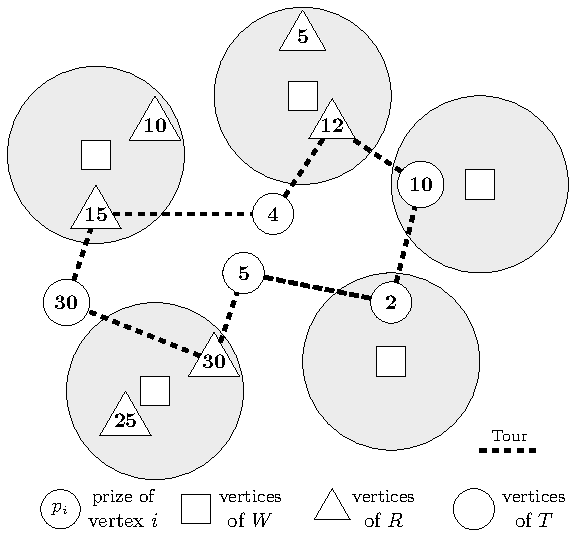
\includegraphics[width=0.45\textwidth]{pcctp-solution.pdf}
	\caption{A feasible solution for a small instance with the value of $PRIZE$ set to 100.}
	\label{fig:pcctp}
\end{figure}

According to \citet{daSilva},  a real-world scenario for the PCCTP may be found in the supply of a tour for itinerant vehicles providing social services. The vertices of $T$ are considered as important cities in an area that are specified as necessary visiting points, whereas the vertices of $R$ refer to optional stop locations. For set $W$, it would contain locations that are difficult to access, and then to serve their respective people, the vehicle would have to pass through a location ($T$ or $R$) of up to $D$ units of distance. For the vehicle release to be worthwhile, a minimum quantity of people must be attended. As a result, each vertex's prize represents the population of each city to be visited, and the total prize to be collected refers to the minimum total number of residents to be serviced.



The remainder of the paper is structured as follows.  Section \ref{sec:grasp} presents a short review of the literature on PCCTP and provides details of the state-of-the-art heuristic. Section \ref{sec:datamining} details the proposed data mining approaches. Computational results are shown and analysed in Section \ref{sec:computationalresults}. Finally, in Section \ref{sec:conclusions} the conclusions are drawn and some future works are pointed out.


\section{GRASP-GENIUS-RVND: The state-of-the-art heuristic}

\label{sec:grasp}

Few authors have discussed the PCCTP before and some solution methods have been presented. \citep{lyra2004problema} introduced the PCCTP and as solution methods, proposed a mathematical formulation the makes use of flow constraints to eliminate sub-tours, and a GRASP-based heuristic  \citep{grasp03}   associated with a VNS (Variable Neighbourhood Search) metaheuristic \citep{mladenovic97}.  Also, a path-relinking strategy was used as an intensification component for trying to improve solutions.

Next, \citet{silva2009problema} introduced  six new heuristics,  which are based on the ILS (Iterated Local Search) metaheuristic and evolutionary algorithms. Finally, \citet{daSilva} proposed GRASP-based heuristic embedded with a GENIUS \citep{genius} and Random VND \citep{mladenovic12} heuristics (GRASP-GENIUS-RVND). In this heuristic, the GENIUS performed the initial solution generation, while RVND was responsible for the local search of the GRASP. As far as the authors know, the GRASP-GENIUS-RVND is the state-of-the-art heuristic for the PCCTP, in terms of quality solution and CPU time.


% The PCCTP is relatively new in the literature and there are two mathematical formulations describing it. The first one was proposed by \citet{lyra2004problema} along with the problem and makes use of constraints based on flow to eliminate sub-tours in the solution. The second one was proposed by \citet{silva2009problema}, and it is based on multi-flow constraints to handle sub-tours in the solution. 

% Since PCCTP is an NP-Hard problem, some heuristics have been proposed. \citet{lyra2004problema} proposed a heuristic based on GRASP combined with a variation of the VNS (Variable Neighbourhood Search) metaheuristic \cite{hansen1997variable}. Its heuristic approach also includes a path-relinking technique as an improving solutions component.
% In the following, \citet{silva2009problema} proposed new six heuristic methods, in which five of them are based on the ILS (Iterated Local Search) meta-heuristic \cite{lourencco2003iterated},
% and one is an evolutionary heuristic. \citet{silva2009problema} conducted experiments on test problems proposed in his work and the ILS-RDM-CI was the one with the best overall performance. 





% maximum number of disturbances is reached.



% \section{Heuristic approaches}
% As will be shown in Section \ref{sec:results}, although the proposed new formulation allows for the unprecedented resolution of several instances of the literature, there are still those that are not possible to be solved exactly, either due to the need for a long execution time or for problems related to the lack of memory of the computer. Therefore, this work also proposes three new hybrid heuristics: one hybridization with ILP (MPO\_S) and two hybridizations with data mining (DM-GRASP and MDM-GRASP).


\subsection{GRASP-GENIUS-RVND}

% The most recent work for PCCTP refers to the GRASP-GENIUS-RVND heuristic presented in \citet{daSilva}, which is  the state-of-the-art for obtaining approximate solutions. 

The GRASP-GENIUS-RVND \citep{daSilva} is based on the GRASP (Greedy Randomised Adaptive Search Procedure) metaheuristic \citep{grasp03}. GRASP is based on a multi-start strategy, in which many initial solutions are generated through repeated applications of a semi-greedy process. At each multi-start iteration, given a constructed solution $S$, its neighbourhood $N(S)$ is explored by a local search, in order to find a better solution. The iterative process of performing the two phases, initial solution generation, and local search, is interrupted according to a stopping criterion, which can be a maximum number of interactions, a target solution value, or timeout.



% The GRASP metaheuristic is executed iteratively, and each iteration is composed of two phases: construction and local search. A feasible solution $S$ is generated in the construction phase, and then its Neighbourhood $N(S)$ is explored by a local search, in order to find a better solution. This iterative process is repeated until a stop criterion is reached, that can be a limited number of iterations allowed, a number of iterations without solution improvement, among others. The best solution found in all iterations $S^*$ is returned. 

\citet{daSilva} developed the solution generation phase based on the GENIUS heuristic \citep{genius} adapted for the PCCTP, while in the other phase, some moves were devised and combined in an RVND (Random Variable neighbourhood Descent) framework \citep{mladenovic97}.


% \subsubsection{GENIUS}

% The GENIUS heuristic \citep{genius} is divided into two steps: a construction approach, the GENI step (Generalised Insertion), and a method of improvement, the Unstringing and Stringing (US) step. The GENI is a generalised insertion-based method whose main characteristic is that the evaluation of the possible insertions of a vertex is not essentially limited to a position between consecutive vertices. 
% The US step consists, at each iteration, in removing
% one vertex from the tour and re-inserting it in another position with a view
% of improving the current solution. This procedure stops when there is no more
% possibility of improvements.

% In the construction phase, a partial route is generated by three vertices randomly chosen from $T$, and then, as long as there is a vertex of $T$ outside the tour, the $PRIZE$ is not reached and there is any uncovered vertex $w \in W$, the following steps are performed: i) a candidate list (CL) is created containing all vertices outside the route; ii) a  restricted candidate list (RCL) is formed by the best-quality vertices from CL; iii) a vertex is selected at random from the RCL and inserted in the using the GENI procedure; and iv) one tries to improve the route by performing the US method. The pseudo-code of the GENIUS procedure is presented in Algorithm \ref{alg:genius_PCCTP}.

% A vertex is inserted into the RCL if its incremental cost is inferior to the threshold $c^{min} + (\alpha \times (c^{max} - c^{min}))$, where $c^{min}$ and $c^{max}$ are, respectively, the smallest and the largest incremental costs in CL. The greedy parameter $\alpha \in [0,1]$ indicates how greedy the heuristic is, the higher the value of $\alpha$ the greedier.

% For calculating the incremental cost, we used the following greedy function, which considers the insertion of a vertex $k$ between two other vertices $i$ and $j$.

% \begin{eqnarray}
% g(k) = \displaystyle \min_{i,j \in S : i \neq j} \left(c_{ik} + c_{kj}  - c_{ij}\right) \label{custo_inc}
% \end{eqnarray}

% \noindent where $c_{ij}$, $c_{ik}$ and $c_{kj}$ are, respectively, the cost of the edges $(i,j)$, $(i,k)$ and $(k,j)$.

% \begin{algorithm}[ht]
% 	%	\algsetup{linenosize=\scriptsize}
% 	\caption{\hspace{-1mm}: GENIUS($seed$,$\alpha$)}
% 	\label{alg:genius_PCCTP}
% 	%	{\footnotesize
% 		{\footnotesize
% 	\begin{algorithmic}[1]
% 		%			\REQUIRE $seed$, $\alpha$
% 		\STATE $i, j, k \gets \texttt{SelectRandom}(T,seed)$;
% 		\STATE $S \gets \cup$ $\{i, j, k\}$;
% 		\STATE $LC \gets V$;
% 		\STATE $LC \gets LC \setminus \{i,j,k\}$
% 		\WHILE{$(\exists$ $t \in T$ : $t \notin S )$ \textbf{or} $(\exists$ not covered $w \in W\space)$ \textbf{or} (\textit{PRIZE} not collected) }
% 		\STATE $LRC \gets \texttt{setLRC}(LC, \alpha)$;
% 		\STATE $v \gets \texttt{SelectRandom}(LRC,seed)$;
% 		\STATE $GENI(S,v)$;
% 		\STATE $LC \gets LC \backslash {v} $;
% 		\ENDWHILE
% 		\STATE $US(S)$; \textit{//tour improvement}\\
% 		\RETURN $S$;
% 	\end{algorithmic}
% 		}
% \end{algorithm}

% \subsubsection{RVND}
% After the construction phase of GRASP, the built solution goes through a local search performed by the Random VND method \citep{mladenovic97}. Proposed by \citet{mladenovic97}, the VND is a local search metaheuristic that uses different neighbourhood structures. Given an ordered list of neighbourhoods, the VND starts by exploring the first neighbourhood of $S$, $N^k(S)$, and if a better solution is not found, the next neighbourhood $N^{(k + 1)} (S) $ is explored. Otherwise, it returns to the first neighbourhood on the list. The algorithm stops when all neighbourhood structures are explored, returning the best solution found. In this work, we have used the RVND instead of the conventional VND, where there is no fixed sequence of neighbourhoods because they are randomly reorganised on each application of the local search.

% The RVND is detailed in the pseudo-code of Algorithm \ref{alg:vnd}, and it starts by shuffling the list of neighbourhood structures. Then, we can see that the counter $k$ is incremented by one to try the next neighbourhood if the current solution is not improved. Otherwise, the  local optimal solution for the current neighbourhood is obtained, and $k$ is set to 1 so that the loop restarts for the newly accepted solution. When none of the neighbours are able to improve $S$, i.e., $k > k_{max}$, the best current solution is returned.

% For the RVND, \citet{daSilva} used 15 neighbourhood structures, which are based on classical movements for the TSP as \textit{swap} and \textit{shift}, and well-known heuristics such as GENIUS and Cheapest Insertion.


% \begin{algorithm}
% 	\caption{\hspace{-1mm}: RVND($S, N$).}
% 	\label{alg:vnd}
% 		{\footnotesize
% 	\begin{algorithmic}[1]		
% 		\STATE  Set a random order for the neighbourhood structures in $N$	
% 		\STATE $k \gets 1$
% 		\WHILE {$k \leq k\_max$}
% 		\STATE $S' \gets firstImprovingSolution(N^{(k)}(S))$;
% 		\IF{\textit{S' is better than S}}
% 		\STATE $S \gets S'$;
% 		\STATE $k \gets 1$;
% 		\ELSE
% 		\STATE $k \gets k + 1$;
% 		\ENDIF
% 		\ENDWHILE
% 		\RETURN $S$
% 	\end{algorithmic}	
% }
% \end{algorithm}


\subsubsection{GENIUS}

The GENIUS heuristic \citep{genius} is implemented with  two steps: a construction approach, the GENI step (Generalized Insertion), and an improvement procedure, the Unstringing and Stringing (US) step. 

GENI is method with a generalized insertion. Its main feature is that the evaluation of possible insertion of vertices is basically not limited to the positions between consecutive vertices.
The US step involves removing a vertex from the tour and reinserting it in another position, in each iteration, to improve the current solution. When there are no more possibilities for improvement, this process stops.

% The GENI is a generalized insertion-based method whose main characteristic is that the evaluation of the possible insertions of a vertex is not essentially limited to a position between consecutive vertices. 
% The US step consists, at each iteration, of removing
% one vertex from the tour and re-inserting it in another position with a view
% of improving the current solution. This procedure stops when there is no more
% possibility of improvements.

In the construction phase, we start by randomly selecting three vertices from $T$ to generate a partial tour. Then, as long as there are vertices of $T$ outside the tour, the $PRIZE$ has not been reached, and there are any uncovered vertices $w \in W $, we  perform the following steps: i) create a candidate list (CL), which contains all vertices outside the tour; ii) obtain a restricted candidate list (RCL) which is composed of the best quality vertices from CL; iii) a vertex is randomly selected from RCL and inserted in the tour by a GENIUS procedure; iv) try to improve the tour by applying the US method. The pseudo-code of the GENIUS process is given in the algorithm \ref{alg:genius_PCCTP}.

According to \citet{daSilva}, if the incremental cost of a vertex is lower than the threshold $c^{min} + (\alpha \times (c^{max}-c^{min}))$, the vertex is inserted into in the RCL, in which $c^{min}$ and $c^{max}$ are the smallest and largest incremental costs in CL, respectively. The greedy parameter $\alpha \in [0,1]$ represents the greedy degree of the heuristic, the lower the value of $\alpha$ is, the lower the greedy.

% For calculating the incremental cost, we used the following greedy function, which considers the insertion of a vertex $k$ between vertices $i$ and $j$.

We have used the following  greedy function (Equation \ref{custo_inc} to compute the incremental cost, which takes into account the insertion of a vertex $v$ between vertices $i$ and $j$.

\begin{flalign}
g(v) = \displaystyle \min_{i,j \in V : i \neq j} \left(c_{iv} + c_{vj}  - c_{ij}\right) \label{custo_inc}
\end{flalign}

\noindent where $c_{ij}$, $c_{iv}$ and $c_{vj}$ are the costs of the edges $(i,j)$, $(i,v)$ and $(v,j)$, respectively.

\begin{algorithm}[ht]
	%	\algsetup{linenosize=\scriptsize}
	\caption{\hspace{-1mm}: GENIUS($seed$,$\alpha$)}
	\label{alg:genius_PCCTP}
	%	{\footnotesize
		{\footnotesize
	\begin{algorithmic}[1]
		%			\REQUIRE $seed$, $\alpha$
		\STATE $i, j, k \gets \texttt{SelectRandom}(T,seed)$;
		\STATE $S \gets \cup$ $\{i, j, k\}$;
% 		\STATE $CL \gets V$;
		\STATE $CL \gets V \setminus \{i,j,k\}$
		\WHILE{$(\exists$ $t \in T$ : $t \notin S )$ \textbf{or} $(\exists$ not covered $w \in W\space)$ \textbf{or} (\textit{PRIZE} not collected) }
		\STATE $RCL \gets \texttt{setRCL}(CL, \alpha)$;
		\STATE $v \gets \texttt{SelectRandom}(RCL,seed)$;
		\STATE $GENI(S,v)$;
		\STATE $CL \gets CL \backslash {v} $;
		\ENDWHILE
		\STATE $US(S)$; \textit{//tour improvement}\\
		\RETURN $S$;
	\end{algorithmic}
		}
\end{algorithm}

\subsubsection{RVND}
Following the GRASP construction phase, the generated solution is subjected to a local search using the Random VND technique \citep{mladenovic12}. The VND is a local search metaheuristic proposed by \citet{mladenovic97} that employs several neighbourhood structures. Given an ordered list of neighbourhoods, initially, the VND explores the first neighbourhood of $S$, $N^k(S)$, and if a better solution cannot be discovered, the next $N^{(k + 1)}(S) $  neighbourhood is investigated. Otherwise, it will go back to the first neighbourhood on the list. When all neighbourhood structures have been explored, the algorithm comes to a halt and returns the best solution found. For their heuristic, \citet{daSilva} used the RVND instead of the traditional VND in which there is no neighbourhood order.


% After the construction phase of GRASP, the built solution goes through a local search performed by the Random VND method \citep{SUBRAMANIAN20101899}. Proposed by \citet{mladenovic97}, the VND is a local search metaheuristic that uses different neighbourhood structures. Given an ordered list of neighbourhoods, the VND starts by exploring the first neighbourhood of $S$, $N^k(S)$, and if a better solution is not found, the next neighbourhood $N^{(k + 1)}(S) $ is explored. Otherwise, it returns to the first neighbourhood on the list. The algorithm stops when all neighbourhood structures are explored, returning the best solution found. In this work, we have used the RVND instead of the conventional VND, where there is no ordering of neighbourhoods. 


The RVND is detailed in the pseudo-code of Algorithm \ref{alg:vnd}, and it starts by shuffling the list of neighbourhood structures. Then, we can see that the counter $k$ is incremented by one to try the next neighbourhood if the current solution is not improved.
Otherwise, the current neighbourhood's local optimal solution is achieved, and $k$ is set back to 1 for restarting the loop for the newly accepted solution.
When there is no chance of improving $S$, that is, $k > k_{max}$, one returns the best current solution.

RVND is described in detail in the pseudo-code of Algorithm \ref{alg:vnd}. It first scrambles the list of neighbourhood structures. Then, we can see that if the current solution is not improved, the counter $k$ will increase by 1 to try the next neighbourhood. Otherwise, we obtain the local optimal solution of the current neighbourhood and we set $k$ to 1 to restart the loop for the newly accepted solution. When there are no neighbors to improve $S$, that is, $k> k_{max}$, the algorithm returns the current best solution.



% For the RVND, we used  the 15 neighbourhood structures presented in \citet{daSilva}, which are based on classical movements for the TSP as \textit{swap} and \textit{shift}, and heuristics as GENIUS and Cheapest Insertion.

For RVND, we have used the 15 neighbourhood structures introduced in \citet{daSilva}, which are based on TSP's classic movements \textit{swap} and \textit{shift}, as well as heuristics as GENIUS and the cheapest insert.


\begin{algorithm}
	\caption{\hspace{-1mm}: RVND($S, N$)}
	\label{alg:vnd}
		{\footnotesize
	\begin{algorithmic}[1]		
		\STATE  Set a random order for the neighbourhood structures in $N$	
		\STATE $k \gets 1$
		\WHILE {$k \leq k\_max$}
		\STATE $S' \gets firstImprovingSolution(N^{(k)}(S))$;
		\IF{\textit{S' is better than S}}
		\STATE $S \gets S'$;
		\STATE $k \gets 1$;
		\ELSE
		\STATE $k \gets k + 1$;
		\ENDIF
		\ENDWHILE
		\RETURN $S$
	\end{algorithmic}	
}
\end{algorithm}



\section{Data mining}

\label{sec:datamining}

In a database composed of transactions, in which each transaction corresponds to a set of elements of the application domain, different relationships between data can be extracted in the form of sets of frequent items (patterns). A set of items, which is a subset of items in the application domain, is extracted if its support, a percentage indicator of its occurrence in the data set, is greater than or equal to a certain minimum support. This set is called a set of frequent items.

Thus, the problem of mining frequent item sets is to identify all frequent item sets in the database concerning certain minimum support. In addition, sets of maximal frequent items can also be mined, where a set of maximal frequent items corresponds to a set of frequent items that are not a subset of any other set of frequent items.


Consider $ E = \{e_1, e_2, e_3 ..., e_n \} $ as a set of application elements, a transaction $ t $ as a subset of $ E $, and a database $ D $ as a set of transactions. A set of frequent items $ F $, with support $ sup $, is a subset of $ E $ that occurs in at least $ (sup \times 100) \% $ of transactions in $ D $. Therefore, the identification of all sets of frequent items in $ D $, with minimal support ($ sup_{min} $) defined as an input parameter, is the frequent item-set mining (FIM) problem, in which several efficient algorithms have been proposed in the literature to solve it, including Apriori \cite{agrawal1994fast} and FP-Growth \cite{han2000mining}. The FP-max* \footnote{is available at http://fimi.uantwerpen.be/} \cite{goethals04} algorithm was proposed to efficiently mine sets of maximal frequent items \cite{grahne2003efficiently}.
	
%For exemplification purposes, let E ={1, 2, 3, 4, 5} be the set of all elements of the applicationdomain and supminequal to 80%. Consider a dataset D composed of five transactions, for example,D ={{1, 2, 3, 4, 5}, {1, 2, 3, 5}, {2, 3, 4, 5}, {1, 2, 5}, {2, 3, 4}}. By applying an FIM technique in D,the frequent itemsets extracted are {2}, {3}, {5}, {2, 3},and{2, 5}, since they occur in, at least, 80%of all transactions of D. Note that, in case of mining maximal frequent itemsets, only {2, 3} and{2, 5} are extracted as these itemsets are not subsets of any frequent itemset.
\subsubsection{GRASP hybridisation with data mining}
GRASP, in its original form, does not have any type of long-term memory. This fact is due to its iterative and multistart nature, with totally independent iterations that, at each iteration, start a new random search process \cite{aloise2011adaptive}.

In the literature, there are proposals for strategies that maintain information from previous iterations, to assist the search process in future iterations \cite{fleurent1999improved, italo, rochat1995probabilistic, plastino2011hybrid, plastino2014adaptive, ribeiro2006hybridization}. Regarding the GRASP metaheuristic, a combination with data mining was proposed by \citet{ribeiro2006hybridization} to solve the Set Packing Problem. This approach has been successful in achieving promising results not only in terms of solution quality but also in execution time. The basic idea of incorporating data mining is to extract patterns found in sub-optimal solutions, to then efficiently guide the search for better solutions.


The strategy adopted by \citet{ribeiro2006hybridization} was to divide the original GRASP into two parts. The first part is responsible for obtaining a set of good quality solutions (elite set). Then, the data mining process is applied to this elite set, in order to extract a set of patterns. The second part uses, in each iteration, a pattern from the set of patterns extracted to generate an initial solution, through an adapted construction method. Since this strategy obtained satisfactory results in solving the problem addressed in \citet {ribeiro2006hybridization} and, in others in the literature \cite{santos2005hybrid, guerine2020hybrid, barbalho2013, guerine14}, we have decided to adopt it for approaching the PCCTP.

Initially, GRASP with DM was successfully applied to optimisation problems that represent solutions as sets of elements. Mining item sets for such a category of problems was straightforward since item sets are sets of elements. However, this technique cannot be directly employed, when the order of the elements is relevant in the solution.

In \citet{guerine14}, a strategy based on GRASP with DM was proposed for a variant of the traveling salesman problem (TSP), to deal with the element order problem as follows: instead of intuitive vertex mining, which are the solution elements, this technique considered arc mining, which naturally maintains the order of the vertices. Basically, each pair of vertices $ (i, j) $, that is, an arc of a solution, is mapped to a unique identifier that represents it ($a_{ij}$). This mapping is performed for all solutions in the elite set, that is, transforming the solutions into sets of elements, which are easily treated by an FIM technique.


In \citet{guerine14}, the solutions were mapped as follows. Given a pair of sequential vertices, represented by the edge $ (i, j) $, the unique identifier that represents that edge is calculated by $ a_{ij} = (i \times | V |) + j $, where $ | V | $ is the number of vertices of the problem. Once the pattern is extracted, a reverse process to the mapping is performed as follows. From the identifier $ a_{ij} $, we have $ i = (a_{ij} $ $ div $ $ | V |) $ and $ j = (a_{ij} $ $ mod $ $ | V |) $ , where $ div $ and $ mod $ are the mathematical operators used to obtain, respectively, the quotient and the rest of the division.

As the PCCTP solutions are also influenced by the order of the vertices, the \citet {guerine14} mapping strategy was adopted in this work. In the next section, we present the hybrid heuristic proposal, which combines the GRASP-GENIUS-RVND with data mining.

\subsection{DM-GRASP}

The DM-GRASP, proposed in this work, is based on the strategy of \citet{guerine14}, which is divided into two phases, with half the total number of iterations each, separated by the data mining process. In the first phase, which is identical to the original GRASP-GENIUS-RVND heuristic, the best solutions found are stored in an elite set $M$ with size $cap$. A solution $S$ is eligible to be inserted into $M$ if either $S$ is better than the worst solution of $M$, or if $M$ is not full. Furthermore, $M$ does not allow for identical solutions.

After the first phase, the data mining process runs and generates a set of patterns with support greater than or equal to certain minimum support $sup_{min}$. Then, the second phase uses, at each iteration, a pattern from the set of patterns to build an initial solution through an adapted constructive procedure. In the end, the best solution found is returned. The DM-GRASP pseudo-code for the PCCTP is presented in the pseudo-code of Algorithm \ref{alg:dm-grasp} .

In line 1, all sets and variables of the algorithm are initialised. In the first phase of the strategy (lines 2 to 10), which corresponds to the first half of the iterations, the algorithm remains the same as the original GRASP-GENIUS-RVND, except for the presence of the function \texttt{UpdateEliteSet}($M, S'', cap$) (line 8). This function inserts $S''$, which is a solution obtained by RVND, into $M$ if $S''$ is unique in $M$ and its cost is less than the worst solution in $M$. After the end of the first $k$ iterations, in line 11 the mining procedure extracts $t$ patterns from the elite set, and these patterns are inserted in descending order of size (number of edges) in the pattern set. In this work, pattern extraction is performed by the FP-max* algorithm \cite{goethals04}, which is an efficient implementation for extracting sets of maximal frequent items.

In the second phase of the algorithm (lines 12 to 20), which performs the second half of the iterations, an adapted constructive procedure replaces the original constructive procedure (line 14). This adapted procedure, which is explained
later, is executed after selecting the next largest pattern by means of a selection \textit{round-robin} \cite{furnkranz2001round} from $patterns\_set$, and the identifiers contained in the patterns are mapped back to the form of edges, as explained above. Then, the remaining lines of the second part are equal to their respective parts of the original GRASP-GENIUS-RVND. At the end of all iterations, the best solution $S$ is returned (line 21).



\begin{algorithm}[!h]
	\caption{\hspace{-1mm}: \textbf{DM-GRASP}($maxIt, seed, t, cap, \alpha, sup_{min}$)}
	\label{alg:dm-grasp}
	{\footnotesize
		\begin{algorithmic}[1]		
			\STATE $S\gets \emptyset$; $f(S) \gets \infty$; $M \gets \emptyset$; $k \gets 1$; 
			\WHILE{$k \leq maxIt/2$}
			\STATE $S' \gets \texttt{GENIUS} (seed, \alpha)$;  \COMMENT{Construction phase }
			\STATE $S'' \gets \texttt{RVND} (S', seed)$; \COMMENT{Local search phase}
			\IF{$f(S'') \leq f(S)$}
			\STATE $S \gets S''$;
			\ENDIF
			\STATE \texttt{UpdateEliteSet}($M, S'', cap$);
			\STATE $k \gets k +1$;
			\ENDWHILE
			\STATE	$patterns\_set \gets$ \texttt{mine}($M, cap, t, sup_{min}$)
			\WHILE{$k \leq maxIt$}
			\STATE $padrao \gets $\texttt{selectLargestNextPattern}($patterns\_set$); 
			\STATE $S' \gets$ \texttt{GENIUS\_adapted}($seed, \alpha, pattern$);
			\STATE $S'' \gets \texttt{RVND} (S', seed)$;
				\IF{$f(S'') \leq f(S)$}
			\STATE $S \gets S''$;
			\ENDIF
			\STATE $k \gets k +1$;
			\ENDWHILE
			\RETURN $S$;
		\end{algorithmic}
	}
\end{algorithm}

For the generation of solutions using patterns, an adapted version of the GENIUS heuristic proposed by \citet{daSilva} was used, however, each GENIUS construction no longer starts from a sub-route with three random vertices, but from a mined pattern. The pseudo-code of Algorithm \ref{alg:genius-adaptado}  presents this construction in more detail.

In line 1, the solution $S$ is initialised containing all the edges of the pattern. In line 2, the candidate list is initialised with all problem vertices that are not yet on the route. Then, while $S$ is not complete, a vertex is chosen randomly from a restricted list of candidates, and inserted into the route using the GENI heuristic (lines 4 to 10). Finally, the US refinement heuristic tries to improve $S$ (line 11), which is returned in line 12.


\begin{algorithm}[!h]
	{\small
	\caption{\hspace{-1mm}:  GENIUS\_adapted($seed, \alpha, padrao$)}
	\label{alg:genius-adaptado}
	\begin{algorithmic}[1]			
		\STATE $S \gets pattern$;
		\STATE $CL \gets V \setminus S$
		\STATE \texttt{Evaluate}($CL$);
		\WHILE {$! SolutionComplete(S)$}
			\STATE $RCL \gets buildLRC(\alpha, CL)$;
			\STATE $v \gets choose\_randomly(RCL)$;
			\STATE \texttt{GENI}($S, v$);
			\STATE $CL \gets CL \setminus \{v\}$;
			\STATE \texttt{Evaluate}($CL$);
		\ENDWHILE
		\STATE \texttt{US}($S$);
		\RETURN $S$;
	\end{algorithmic}
}
\end{algorithm}



\subsubsection{MDM-GRASP}
In the DM-GRASP proposal, the data mining procedure is executed only once, exactly after half of the iterations.
In addition to this strategy, this work also proposes and examines another approach, which applies the mining procedure more than once during the execution of the algorithm.

% , based on investigations in the literature \cite{barbalho2013, plastino2014adaptive, plastino09}.

According to the literature \cite{barbalho2013}, running data mining more than once will explore the gradual evolution of the elite set, and allow for the extraction of more refined patterns.
In this new method, mining is applied as soon as $M$ becomes stable and whenever this set is changed and becomes stable again. This last method is called \textit{Multi Data-Mining} GRASP (MDM-GRASP). In the context of this work, $M$ is said to be stable if its set of solutions remains unchanged for a certain number of consecutive $\omega$ iterations, that is, throughout these iterations, no good quality solutions are found that can be inserted in this set.

The pseudo-code of MDM-GRASP is presented in the Algorithm \ref{alg:mdm-grasp}. From lines 2 to 24, as long as a maximum number of $maxIt$ interactions is not reached, the following instructions are executed. From lines 3 to 7, if some data mining procedure has already been performed, then $S'$ is obtained by an adapted construction (line 7), otherwise, the GRASP-GENIUS-RVND construction is applied (line 4) . In line 9, a solution $S''$ is obtained from a local search applied to $S'$. From lines 10 to 12, if the cost of $S''$ is less than the cost of the best current solution $S$, then $S$ is updated. From lines 13 to 17, if $M$ is updated with solution $S''$, then the non-update counter 
($Iter_{sa}$) is reset to zero (line 14), otherwise, this counter is incremented (line 16). From lines 18 to 22, if $M$ is stable, that is, if $Iter_{sa}$ is equal to $\omega$, then the mining procedure is applied (line 19), and this counter is reset to zero (line 20). Finally, the best solution is returned in line 25.


\begin{algorithm}[h]
  {\small
	\caption{\hspace{-1mm}: MDM-GRASP($maxIt, seed, t, cap, \alpha, sup_{min}, \omega$)}	
	\label{alg:mdm-grasp}
	\begin{algorithmic}[1]
		
		\STATE $S \gets \emptyset$; $f^* \gets \infty$;  $M \gets \emptyset$; $k \gets 0$; $did\_mining \gets false$; $Iter_{sa} \gets 0$;
		
%		\WHILE{$!estavel(M)$ e $k < maxIt$}
%		\STATE (Linhas 3 a 9 do Algoritmo \ref{alg:dm-grasp});
%		
%		\ENDWHILE
		
		\WHILE{$k < maxIt$}
			\IF{$did\_mining = false$}
				\STATE $S' \gets \texttt{GENIUS} (seed, \alpha)$; 
			\ELSE
				\STATE $pattern \gets $\texttt{selectNextLargestPattern}($pattern\_set$); 
				\STATE $S' \gets$ \texttt{GENIUS\_adapted}($seed, \alpha, pattern$); 
			\ENDIF
			\STATE $S'' \gets \texttt{RVND} (S', seed)$; 
			\IF{$f(S'') \leq f^*$}
			\STATE $S \gets S''$; $f^* \gets f(S'')$;
			\ENDIF
			\IF {\texttt{updateEliteSet}($M, S'', cap$)}
				\STATE $Iter_{sa} \gets 0$;
			\ELSE
				\STATE $Iter_{sa} \gets Iter_{sa} + 1$;
			\ENDIF
			\IF{$Iter_{sa} = \omega$}
				\STATE $pattern\_set \gets$ \texttt{mine} ($M,cap,t, sup_{min}$);
				\STATE $Iter_{sa} \gets 0$;
				\STATE $did\_mining\gets true$;
			\ENDIF	
			\STATE $k \gets k + 1$;
		\ENDWHILE
		\RETURN {$S$};
		
	\end{algorithmic}
}
\end{algorithm}


\section{Computational results}

\label{sec:computationalresults}

In this section, computational experiments performed with the proposed approaches are presented and compared with the state-of-the-art heuristic. We emphasise that GRASP-GENIUS-RVND original implementation was fully provided by
the authors and is the base of our DM-GRASP and MDM-GRASP. 

For a fair comparison, all heuristics presented were implemented in \textit{C++} language and compiled with \textit{g++ 5.4.0}. The experiments were carried out on an Intel(R) Core i7-6700 CPU\@ 3.40GHz machine with 16GB of RAM. 


\subsection{Instances}

\citet{silva2009problema} proposed the instances utilised in \citet{daSilva} and in this work, which consist of 144 test problems derived from the traveling salesman problem (TSP) accessible at the \citet{reinelt1991tsplib} repository.  The $PRIZE$ is never satisfied with the collection of merely the prizes associated with the vertices from $T$, in order to avoid any instance of the PCCTP from becoming an instance of the covered tour problem (CTP).

The name of the instances are based on their original names from the TSPLIB, with extra information regarding the subsets $R$, $T$, and $W$, as well as the proportion of the total $PRIZE$ to be collected \cite{silva2009problema}. The instance \textit{a280\_R56\_T168\_W56\_50}, for example, contains the following properties: the total number of vertices is 280,  56 of them are optional ($R$), 168 are mandatory ($T$), 56 must be covered ($W$), and 50\% of the total prize must be covered. 

These instances were named according to their original name in the TSPLIB, adding additional information about the subsets $R$, $T$, $W$ and the percentage of prize to be collected, in relation to the total available prize. For example, the instance \textit{brazil58\_R18\_T20\_W20\_25} has the following characteristics: 58 vertices in total; 18 optional vertices $R$; 20 mandatory vertices $T$; 20 vertices to be covered $W$; and 25\% of the total instance prize must be collected. They are publicly available in a  Mendeley repository \citep{pcctspMendely}.

\subsection{Results for the DM-GRASP and MDM-GRASP}

For the DM-GRASP and MDM-GRASP algorithms, the value defined for the parameter $maxIt$ of the state-of-the-art heuristic was kept. For both algorithms, the minimum support was defined as 20\%, as it presents a better cost-benefit ratio between time spent and solution quality, compared to the other values tested (30\%, 40\% and 50\%).

Experiments were carried out with 37 instances, from ten executions for each support configuration, using different seeds for each execution. Support values were only tested from $sup\_min$ = 10\% to 50\%, as with $sup\_min$= 60\% there is no longer any data mining occurrence in any of the tested instances. For the complete results of these experiments, the readers may refer to the Mendeley repository \cite{pcctspMendely}.

After tuning the minimum support to be used, experiments were carried out with the 107 remaining instances of \citet{silva2009problema}. The results of this experiment are presented in Tables \ref{tab:dm-grasp} (DM-GRASP) and \ref{tab:mdm-grasp} (MDM-GRASP). For each strategy, the values of the best solution (BS),  average solution (AS) and average time spent (AT), in seconds,  are presented. The best results are highlighted in bold, and columns $Dif_{as}$ and $Dif_{T}$ refers to the percentage difference between the compared heuristics, respectively, regarding average solution obtained and CPU time spent (see Equations \ref{eq:time} and \ref{eq:as}). In Table \ref{tab:dm-grasp}, Heur1 corresponds to the GRASP-GENIUS-RVND while Heur2 represents the DM-GRASP. In Table \ref{tab:mdm}, Heur1 refers to DM-GRASP and Heur2 represents MDM-GRASP.


\begin{align}
Dif_{T} = 100 \times \frac{(T_{Heur1} - T_{Heur2})}{T_{Heur1}}
\label{eq:time}
\end{align}

% The results of this experiment are presented in Tables 8.14, 8.15, 8.16 and 8.17 (DM-GRASP) and Tables 8.18, 8.19, 8.20 and 8.21 (MDM-GRASP), located in the appendix of this thesis. In the last two columns of these tables, the percentage gain in relation to GRASP-GENIUS-RVND for the DM-GRASP tables and in relation to DM-GRASP for the MDM-GRASP tables are presented.


% {\footnotesize
	\begin{flalign}
	Dif_{BS} = 100 \times \frac{(BS_{Heur1} - BS_{Heur2})}{BS_{Heur1}}
\label{eq:as}
	\end{flalign}
% }

{\scriptsize
	\begin{longtable}{lrrrrrrrr}
		\caption{Comparison between GRASP-GENIUS-RVND and DM-GRASP.}
		\label{tab:dm-grasp}\\
		\hline
		& \multicolumn{3}{c}{GRASP-GENIUS-RVND} & \multicolumn{5}{c}{DM-GRASP} \\
		\cline{2-9}
		%
		%
		Instance & \begin{tabular}[c]{@{}l@{}}BS \end{tabular} & \begin{tabular}[c]{@{}l@{}}AS\end{tabular} & \begin{tabular}[r]{@{}l@{}}AT \end{tabular} & \begin{tabular}[r]{@{}l@{}}BS\end{tabular} & \begin{tabular}[c]{@{}l@{}}AS\end{tabular} & \begin{tabular}[r]{@{}l@{}}AT\end{tabular} & \begin{tabular}[c]{@{}l@{}}$Dif_{BS}$\end{tabular} & \begin{tabular}[c]{@{}l@{}}$Dif_{AT}$\end{tabular} \\
		\hline
		\endhead	
		att48\_R9\_T10\_W29\_25 & \textbf{2291} & \textbf{2291.00} & 0.82 & \textbf{2291} & 2291.27 & \textbf{0.77} & -0.01 & 6.70 \\
		att48\_R9\_T29\_W10\_50 & \textbf{2824} & \textbf{2824.00} & 4.59 & \textbf{2824} & \textbf{2824.00} & \textbf{3.79} & 0.00 & 17.45 \\
		att48\_R16\_T16\_W16\_75 & \textbf{2650} & \textbf{2650.00} & 3.71 & \textbf{2650} & \textbf{2650.00} & \textbf{2.98} & 0.00 & 19.68 \\
		berlin52\_R9\_T11\_W32\_25 & \textbf{4861} & \textbf{4861.00} & 0.86 & \textbf{4861} & \textbf{4861.00} & \textbf{0.78} & 0.00 & 8.32 \\
		berlin52\_R16\_T18\_W18\_50 & \textbf{5186} & \textbf{5186.00} & 4.57 & \textbf{5186} & \textbf{5186.00} & \textbf{4.13} & 0.00 & 9.80 \\
		berlin52\_R9\_T32\_W11\_75 & \textbf{6916} & \textbf{6916.00} & 5.99 & \textbf{6916} & \textbf{6916.00} & \textbf{5.87} & 0.00 & 2.00 \\
		bier127\_R24\_T77\_W26\_25 & \textbf{98597} & 98700.70 & 79.45 & \textbf{98597} & \textbf{98648.20} & \textbf{65.52} & 0.05 & 17.52 \\
		bier127\_R24\_T26\_W77\_50 & \textbf{74745} & \textbf{74745.00} & 22.29 & \textbf{74745} & \textbf{74745.00} & \textbf{16.80} & 0.00 & 24.63 \\
		bier127\_R43\_T42\_W42\_75 & \textbf{98311} & 98390.90 & 101.08 & \textbf{98311} & \textbf{98325.40} & \textbf{88.57} & 0.07 & 12.37 \\
		brazil58\_R18\_T20\_W20\_25 & \textbf{19417} & \textbf{19417.00} & 4.02 & \textbf{19417} & \textbf{19417.00} & \textbf{3.14} & 0.00 & 22.04 \\
		brazil58\_R11\_T35\_W12\_50 & \textbf{23312} & \textbf{23312.00} & 8.12 & \textbf{23312} & \textbf{23312.00} & \textbf{5.90} & 0.00 & 27.26 \\
		brazil58\_R11\_T12\_W35\_75 & \textbf{20466} & \textbf{20466.00} & 1.75 & \textbf{20466} & \textbf{20466.00} & \textbf{1.43} & 0.00 & 18.09 \\
		brg180\_R36\_T36\_W108\_25 & \textbf{550} & \textbf{550.00} & 22.64 & \textbf{550} & \textbf{550.00} & \textbf{20.72} & 0.00 & 8.52 \\
		brg180\_R60\_T60\_W60\_50 & \textbf{2360} & \textbf{2360.00} & \textbf{134.29} & \textbf{2360} & \textbf{2360.00} & 135.35 & 0.00 & -0.79 \\
		brg180\_R36\_T108\_W36\_75 & \textbf{2210} & \textbf{2211.00} & 185.08 & \textbf{2210} & 2215.00 & \textbf{180.94} & -0.18 & 2.23 \\
		ch130\_R44\_T43\_W43\_25 & \textbf{4383} & \textbf{4383.00} & 21.78 & \textbf{4383} & 4383.90 & \textbf{18.96} & -0.02 & 12.95 \\
		ch130\_R26\_T26\_W78\_50 & \textbf{4139} & \textbf{4139.00} & 16.65 & \textbf{4139} & \textbf{4139.00} & \textbf{12.46} & 0.00 & 25.21 \\
		ch130\_R26\_T78\_W26\_75 & \textbf{5287} & \textbf{5303.80} & 87.47 & 5304 & 5306.50 & \textbf{72.20} & -0.05 & 17.46 \\
		ch150\_R50\_T50\_W50\_25 & \textbf{4778} & 4800.20 & 58.63 & \textbf{4778} & \textbf{4797.80} & \textbf{42.89} & 0.05 & 26.85 \\
		ch150\_R30\_T90\_W30\_50 & \textbf{5239} & \textbf{5245.50} & 131.38 & \textbf{5239} & 5247.80 & \textbf{103.98} & -0.04 & 20.85 \\
		ch150\_R30\_T30\_W90\_75 & \textbf{4292} & \textbf{4292.00} & 20.33 & \textbf{4292} & \textbf{4292.00} & \textbf{16.51} & 0.00 & 18.77 \\
		d198\_R39\_T40\_W119\_25 & \textbf{10916} & \textbf{10916.00} & 53.19 & \textbf{10916} & \textbf{10916.00} & \textbf{38.57} & 0.00 & 27.49 \\
		d198\_R39\_T119\_W40\_50 & \textbf{13598} & 13602.60 & 448.89 & \textbf{13598} & \textbf{13599.90} & \textbf{367.46} & 0.02 & 18.14 \\
		d198\_R66\_T66\_W66\_75 & \textbf{12907} & \textbf{12924.40} & 534.73 & \textbf{12907} & 12927.90 & \textbf{424.74} & -0.03 & 20.57 \\
		eil51\_R17\_T17\_W17\_25 & \textbf{273} & \textbf{273.00} & 2.51 & \textbf{273} & \textbf{273.00} & \textbf{2.32} & 0.00 & 7.51 \\
		eil51\_R9\_T11\_W31\_50 & \textbf{248} & \textbf{248.00} & 1.03 & \textbf{248} & \textbf{248.00} & \textbf{0.85} & 0.00 & 17.37 \\
		eil51\_R9\_T31\_W11\_75 & \textbf{348} & 348.50 & 5.18 & \textbf{348} & \textbf{348.10} & \textbf{4.96} & 0.11 & 4.30 \\
		eil76\_R14\_T46\_W16\_25 & \textbf{387} & \textbf{387.00} & 12.18 & \textbf{387} & \textbf{387.00} & \textbf{10.26} & 0.00 & 15.76 \\
		eil76\_R24\_T26\_W26\_50 & \textbf{338} & \textbf{338.00} & 10.54 & \textbf{338} & \textbf{338.00} & \textbf{8.20} & 0.00 & 22.21 \\
		eil76\_R14\_T16\_W46\_75 & \textbf{332} & \textbf{332.00} & 2.92 & \textbf{332} & \textbf{332.00} & \textbf{2.58} & 0.00 & 11.47 \\
		eil101\_R19\_T21\_W61\_25 & \textbf{356} & \textbf{356.00} & 7.73 & \textbf{356} & \textbf{356.00} & \textbf{5.99} & 0.00 & 22.53 \\
		eil101\_R19\_T61\_W21\_50 & \textbf{506} & \textbf{506.00} & 38.8 & \textbf{506} & \textbf{506.00} & \textbf{32.53} & 0.00 & 16.15 \\
		eil101\_R33\_T34\_W34\_75 & \textbf{462} & 463.40 & 40.06 & \textbf{462} & \textbf{463.10} & \textbf{37.64} & 0.06 & 6.03 \\
		gr48\_R16\_T16\_W16\_25 & \textbf{3571} & \textbf{3571.00} & 1.82 & \textbf{3571} & \textbf{3571.00} & \textbf{1.39} & 0.00 & 23.95 \\
		gr48\_R9\_T10\_W29\_50 & \textbf{3524} & \textbf{3524.00} & 0.79 & \textbf{3524} & \textbf{3524.00} & \textbf{0.77} & 0.00 & 2.00 \\
		gr48\_R9\_T29\_W10\_75 & \textbf{4415} & \textbf{4415.00} & 4.16 & \textbf{4415} & \textbf{4415.00} & \textbf{3.91} & 0.00 & 5.96 \\
		gr96\_R18\_T58\_W20\_25 & \textbf{42746} & 42749.60 & 30.44 & \textbf{42746} & \textbf{42746.00} & \textbf{25.15} & 0.01 & 17.40 \\
		gr96\_R32\_T32\_W32\_50 & \textbf{35461} & \textbf{35461.00} & 58.09 & \textbf{35461} & \textbf{35461.00} & \textbf{47.67} & 0.00 & 17.95 \\
		gr96\_R18\_T20\_W58\_75 & \textbf{30015} & \textbf{30015.00} & 9.67 & \textbf{30015} & \textbf{30015.00} & \textbf{7.30} & 0.00 & 24.50 \\
		gr120\_R40\_T40\_W40\_25 & \textbf{4301} & \textbf{4301.00} & 27.8 & \textbf{4301} & \textbf{4301.00} & \textbf{19.35} & 0.00 & 30.40 \\
		gr120\_R24\_T72\_W24\_50 & \textbf{5159} & 5163.70 & 60.02 & \textbf{5159} & \textbf{5161.80} & \textbf{49.16} & 0.04 & 18.10 \\
		gr120\_R24\_T24\_W72\_75 & \textbf{4275} & \textbf{4275.00} & 13.73 & \textbf{4275} & \textbf{4275.00} & \textbf{10.25} & 0.00 & 25.38 \\
		gr137\_R26\_T28\_W83\_25 & \textbf{39305} & \textbf{39305.00} & 15.82 & \textbf{39305} & \textbf{39305.00} & \textbf{13.66} & 0.00 & 13.62 \\
		gr137\_R45\_T46\_W46\_50 & \textbf{46122} & \textbf{46122.00} & 180.51 & \textbf{46122} & \textbf{46122.00} & \textbf{137.59} & 0.00 & 23.78 \\
		gr137\_R26\_T83\_W28\_75 & \textbf{58720} & 58778.00 & 116.18 & \textbf{58720} & \textbf{58748.20} & \textbf{90.59} & 0.05 & 22.02 \\
		hk48\_R9\_T29\_W10\_25 & \textbf{9708} & 9708.60 & 3.82 & \textbf{9708} & \textbf{9708.00} & \textbf{3.50} & 0.01 & 8.24 \\
		hk48\_R16\_T16\_W16\_50 & \textbf{7593} & \textbf{7593.00} & 2.11 & \textbf{7593} & \textbf{7593.00} & \textbf{1.99} & 0.00 & 5.82 \\
		hk48\_R9\_T10\_W29\_75 & \textbf{7803} & \textbf{7803.00} & 0.94 & \textbf{7803} & \textbf{7803.00} & \textbf{0.87} & 0.00 & 7.95 \\
		kroA100\_R20\_T20\_W60\_25 & \textbf{10848} & \textbf{10848.00} & 5.39 & \textbf{10848} & \textbf{10848.00} & \textbf{4.67} & 0.00 & 13.29 \\
		kroA100\_R20\_T60\_W20\_50 & \textbf{16544} & \textbf{16544.00} & 34.1 & \textbf{16544} & \textbf{16544.00} & \textbf{28.29} & 0.00 & 17.03 \\
		kroA100\_R34\_T33\_W33\_75 & \textbf{14606} & \textbf{14606.00} & 43.86 & \textbf{14606} & \textbf{14606.00} & \textbf{33.70} & 0.00 & 23.15 \\
		kroA150\_R50\_T50\_W50\_25 & \textbf{14382} & 14453.20 & 115.63 & 14410 & \textbf{14453.10} & \textbf{104.29} & 0.00 & 9.81 \\
		kroA150\_R30\_T30\_W90\_50 & \textbf{12846} & 12964.60 & 41.69 & 12882 & \textbf{12915.00} & \textbf{36.51} & 0.38 & 12.43 \\
		kroA150\_R30\_T90\_W30\_75 & \textbf{21974} & 21991.00 & 166.24 & \textbf{21974} & \textbf{21987.00} & \textbf{130.56} & 0.02 & 21.47 \\
		kroA200\_R40\_T120\_W40\_25 & \textbf{23495} & \textbf{23495.80} & 303.96 & \textbf{23495} & 23497.80 & \textbf{246.14} & -0.01 & 19.02 \\
		kroA200\_R68\_T66\_W66\_50 & \textbf{17297} & 17323.90 & 727.36 & \textbf{17297} & \textbf{17321.70} & \textbf{530.35} & 0.01 & 27.09 \\
		kroA200\_R40\_T40\_W120\_75 & \textbf{15197} & \textbf{15197.00} & 93.34 & \textbf{15197} & \textbf{15197.00} & \textbf{80.03} & 0.00 & 14.26 \\
		kroB100\_R20\_T60\_W20\_25 & \textbf{18406} & \textbf{18406.00} & 29.93 & \textbf{18406} & \textbf{18406.00} & \textbf{25.11} & 0.00 & 16.09 \\
		kroB100\_R34\_T33\_W33\_50 & \textbf{14160} & \textbf{14164.00} & 55.5 & \textbf{14160} & \textbf{14164.00} & \textbf{43.23} & 0.00 & 22.10 \\
		kroB100\_R34\_T33\_W33\_75 & \textbf{14768} & \textbf{14768.00} & 52.13 & \textbf{14768} & \textbf{14768.00} & \textbf{37.30} & 0.00 & 28.44 \\
		kroB150\_R30\_T30\_W90\_25 & \textbf{11467} & \textbf{11477.80} & 23.54 & \textbf{11467} & \textbf{11477.80} & \textbf{20.07} & 0.00 & 14.74 \\
		kroB150\_R50\_T50\_W50\_50 & \textbf{15388} & \textbf{15414.80} & 181.73 & \textbf{15388} & 15418.20 & \textbf{137.35} & -0.02 & 24.42 \\
		kroB150\_R30\_T90\_W30\_75 & \textbf{21489} & \textbf{21541.70} & 138.07 & \textbf{21489} & 21557.50 & \textbf{114.85} & -0.07 & 16.82 \\
		kroB200\_R40\_T120\_W40\_25 & 24030 & 24057.80 & 320.21 & \textbf{23954} & \textbf{24026.50} & \textbf{257.15} & 0.13 & 19.69 \\
		kroB200\_R40\_T40\_W120\_50 & \textbf{14103} & \textbf{14126.60} & 145.33 & 14125 & 14134.20 & \textbf{113.80} & -0.05 & 21.69 \\
		kroB200\_R68\_T66\_W66\_75 & \textbf{19459} & 19493.10 & 614.45 & \textbf{19459} & \textbf{19472.40} & \textbf{469.76} & 0.11 & 23.55 \\
		kroC100\_R20\_T60\_W20\_25 & \textbf{16785} & \textbf{16785.00} & 31.5 & \textbf{16785} & \textbf{16785.00} & \textbf{24.50} & 0.00 & 22.21 \\
		kroC100\_R34\_T33\_W33\_50 & \textbf{13235} & \textbf{13235.00} & 50.06 & \textbf{13235} & \textbf{13235.00} & \textbf{39.18} & 0.00 & 21.73 \\
		kroC100\_R20\_T20\_W60\_75 & \textbf{12582} & \textbf{12582.00} & 11.39 & \textbf{12582} & \textbf{12582.00} & \textbf{7.84} & 0.00 & 31.13 \\
		kroE100\_R20\_T60\_W20\_25 & \textbf{17199} & 17206.50 & 27.83 & \textbf{17199} & \textbf{17199.00} & \textbf{22.99} & 0.04 & 17.40 \\
		kroE100\_R20\_T20\_W60\_50 & \textbf{10586} & \textbf{10586.00} & 10.97 & \textbf{10586} & \textbf{10586.00} & \textbf{7.93} & 0.00 & 27.70 \\
		kroE100\_R34\_T33\_W33\_75 & \textbf{14622} & \textbf{14622.00} & 47.92 & \textbf{14622} & \textbf{14622.00} & \textbf{36.03} & 0.00 & 24.81 \\
		lin105\_R21\_T21\_W63\_25 & \textbf{8893} & \textbf{8893.00} & 7.72 & \textbf{8893} & \textbf{8893.00} & \textbf{5.97} & 0.00 & 22.61 \\
		lin105\_R21\_T63\_W21\_50 & \textbf{11583} & \textbf{11583.00} & 102.19 & \textbf{11583} & \textbf{11583.00} & \textbf{76.52} & 0.00 & 25.12 \\
		lin105\_R35\_T35\_W35\_75 & \textbf{10566} & 10566.20 & 69.05 & \textbf{10566} & \textbf{10566.00} & \textbf{54.54} & 0.00 & 21.01 \\
		pr76\_R14\_T16\_W46\_25 & \textbf{66007} & \textbf{66007.00} & 2.55 & \textbf{66007} & \textbf{66007.00} & \textbf{2.21} & 0.00 & 13.37 \\
		pr76\_R24\_T26\_W26\_50 & \textbf{74539} & 74540.50 & 15.99 & \textbf{74539} & \textbf{74540.00} & \textbf{14.34} & 0.00 & 10.31 \\
		pr76\_R14\_T46\_W16\_75 & \textbf{90862} & \textbf{90862.00} & 16.04 & \textbf{90862} & \textbf{90862.00} & \textbf{13.66} & 0.00 & 14.84 \\
		pr107\_R20\_T65\_W22\_25 & \textbf{40994} & \textbf{40994.00} & 33.53 & \textbf{40994} & \textbf{40994.00} & \textbf{24.82} & 0.00 & 25.99 \\
		pr107\_R20\_T22\_W65\_50 & \textbf{35869} & \textbf{35869.00} & 4.8 & \textbf{35869} & \textbf{35869.00} & \textbf{3.93} & 0.00 & 18.14 \\
		pr107\_R35\_T36\_W36\_75 & \textbf{37292} & 37322.00 & 36.78 & \textbf{37292} & \textbf{37309.20} & \textbf{26.83} & 0.03 & 27.05 \\
		pr124\_R42\_T41\_W41\_25 & \textbf{35465} & \textbf{35465.00} & 61.79 & \textbf{35465} & \textbf{35465.00} & \textbf{51.94} & 0.00 & 15.94 \\
		pr124\_R24\_T75\_W25\_50 & \textbf{49160} & \textbf{49160.00} & 115.84 & \textbf{49160} & 49164.40 & \textbf{87.77} & -0.01 & 24.23 \\
		pr124\_R24\_T25\_W75\_75 & \textbf{34359} & \textbf{34359.00} & 21.25 & \textbf{34359} & \textbf{34359.00} & \textbf{14.65} & 0.00 & 31.08 \\
		pr136\_R26\_T28\_W82\_25 & \textbf{47620} & \textbf{47620.00} & 11.09 & \textbf{47620} & \textbf{47620.00} & \textbf{7.77} & 0.00 & 29.95 \\
		pr136\_R46\_T45\_W45\_50 & \textbf{59445} & 59512.80 & 125.37 & \textbf{59445} & \textbf{59477.10} & \textbf{90.14} & 0.06 & 28.10 \\
		pr136\_R26\_T82\_W28\_75 & \textbf{78624} & \textbf{78629.80} & 113.31 & \textbf{78624} & 78653.60 & \textbf{82.56} & -0.03 & 27.14 \\
		pr144\_R28\_T87\_W29\_25 & \textbf{46940} & \textbf{46940.00} & 89.39 & \textbf{46940} & 46944.80 & \textbf{64.67} & -0.01 & 27.65 \\
		pr144\_R28\_T29\_W87\_50 & \textbf{30294} & \textbf{30294.00} & 18.9 & \textbf{30294} & \textbf{30294.00} & \textbf{14.97} & 0.00 & 20.79 \\
		pr144\_R48\_T48\_W48\_75 & \textbf{43713} & \textbf{43726.50} & 155.46 & \textbf{43713} & 43743.20 & \textbf{125.64} & -0.04 & 19.19 \\
		pr152\_R50\_T51\_W51\_25 & \textbf{50667} & \textbf{50667.20} & 80.99 & \textbf{50667} & 50667.30 & \textbf{61.45} & 0.00 & 24.13 \\
		pr152\_R29\_T92\_W31\_50 & \textbf{61068} & \textbf{61068.00} & 291.48 & \textbf{61068} & \textbf{61068.00} & \textbf{216.31} & 0.00 & 25.79 \\
		pr152\_R29\_T31\_W92\_75 & \textbf{49110} & \textbf{49110.00} & 49.12 & \textbf{49110} & \textbf{49110.00} & \textbf{31.83} & 0.00 & 35.19 \\
		rat99\_R19\_T20\_W60\_25 & \textbf{792} & \textbf{792.00} & 6.35 & \textbf{792} & \textbf{792.00} & \textbf{5.41} & 0.00 & 14.89 \\
		rat99\_R33\_T33\_W33\_50 & \textbf{847} & \textbf{847.00} & 24.65 & \textbf{847} & \textbf{847.00} & \textbf{20.24} & 0.00 & 17.88 \\
		rat99\_R19\_T60\_W20\_75 & \textbf{1017} & \textbf{1017.00} & 38.08 & \textbf{1017} & \textbf{1017.00} & \textbf{30.74} & 0.00 & 19.27 \\
		rat195\_R65\_T65\_W65\_25 & \textbf{1605} & 1609.10 & 344.38 & \textbf{1605} & \textbf{1606.80} & \textbf{249.12} & 0.14 & 27.66 \\
		rat195\_R39\_T39\_W117\_50 & \textbf{1199} & \textbf{1199.00} & 79.22 & \textbf{1199} & \textbf{1199.00} & \textbf{54.56} & 0.00 & 31.13 \\
		rat195\_R39\_T117\_W39\_75 & 1929 & 1938.00 & 378.31 & \textbf{1928} & \textbf{1933.80} & \textbf{286.81} & 0.22 & 24.19 \\
		rd100\_R34\_T33\_W33\_25 & \textbf{5552} & \textbf{5552.00} & 16.36 & \textbf{5552} & \textbf{5552.00} & \textbf{11.84} & 0.00 & 27.59 \\
		rd100\_R20\_T60\_W20\_50 & \textbf{6619} & 6644.80 & 32.46 & \textbf{6619} & \textbf{6635.90} & \textbf{26.44} & 0.13 & 18.54 \\
		rd100\_R20\_T20\_W60\_75 & \textbf{5421} & \textbf{5421.00} & 6.21 & \textbf{5421} & \textbf{5421.00} & \textbf{5.37} & 0.00 & 13.54 \\
		si175\_R35\_T35\_W105\_25 & \textbf{4845} & 4850.20 & 71.29 & \textbf{4845} & \textbf{4847.60} & \textbf{65.79} & 0.05 & 7.71 \\
		si175\_R35\_T105\_W35\_50 & \textbf{7011} & 7039.00 & 404.75 & \textbf{7011} & \textbf{7032.40} & \textbf{388.96} & 0.09 & 3.90 \\
		si175\_R59\_T58\_W58\_75 & 8430 & 8447.70 & 379.09 & \textbf{8428} & \textbf{8443.10} & \textbf{375.49} & 0.05 & 0.95 \\
		st70\_R14\_T14\_W42\_25 & \textbf{419} & \textbf{419.00} & 2.27 & \textbf{419} & \textbf{419.00} & \textbf{1.75} & 0.00 & 22.71 \\
		st70\_R14\_T42\_W14\_50 & \textbf{554} & \textbf{554.00} & 13.92 & \textbf{554} & \textbf{554.00} & \textbf{11.34} & 0.00 & 18.52 \\
		st70\_R22\_T24\_W24\_75 & \textbf{505} & \textbf{505.00} & 9.39 & \textbf{505} & \textbf{505.00} & \textbf{8.44} & 0.00 & 10.13 \\
		u159\_R31\_T96\_W32\_25 & \textbf{35442} & \textbf{35442.00} & 86.73 & \textbf{35442} & \textbf{35442.00} & \textbf{66.29} & 0.00 & 23.57 \\
		u159\_R31\_T32\_W96\_50 & \textbf{28613} & \textbf{28613.00} & 27.23 & \textbf{28613} & \textbf{28613.00} & \textbf{19.05} & 0.00 & 30.06 \\
		u159\_R53\_T53\_W53\_75 & \textbf{33015} & \textbf{33072.00} & 132.21 & \textbf{33015} & \textbf{33072.00} & \textbf{106.33} & 0.00 & 19.57 \\
		a280\_R94\_T93\_W93\_25 & \textbf{1717} & 1724.60 & 747.75 & 1718 & \textbf{1722.50} & \textbf{644.92} & 0.12 & 13.75 \\
		a280\_R56\_T168\_W56\_50 & \textbf{1996} & \textbf{2001.10} & 1208.35 & 1998 & \textbf{2001.10} & \textbf{1024.14} & 0.00 & 15.24 \\
		a280\_R56\_T56\_W168\_75 & \textbf{1647} & \textbf{1652.00} & 209.48 & \textbf{1647} & \textbf{1652.00} & \textbf{109.35} & 0.00 & 47.80 \\
		gil262\_R51\_T53\_W158\_25 & \textbf{1465} & 1471.30 & 226.15 & \textbf{1465} & \textbf{1468.20} & \textbf{153.66} & 0.21 & 32.05 \\
		gil262\_R88\_T87\_W87\_50 & \textbf{1678} & 1683.10 & 522.83 & \textbf{1678} & \textbf{1682.10} & \textbf{460.43} & 0.06 & 11.94 \\
		gil262\_R51\_T158\_W53\_75 & \textbf{1988} & \textbf{1996.90} & 1383.03 & 1989 & 1999.50 & \textbf{1300.50} & -0.13 & 5.97 \\
		gr202\_R39\_T122\_W41\_25 & \textbf{32162} & 32185.40 & 404.52 & \textbf{32162} & \textbf{32185.20} & \textbf{293.56} & 0.00 & 27.43 \\
		gr202\_R68\_T67\_W67\_50 & \textbf{28706} & 28747.00 & 886.79 & 28723 & \textbf{28741.70} & \textbf{719.21} & 0.02 & 18.90 \\
		gr202\_R39\_T41\_W122\_75 & \textbf{25905} & \textbf{25905.00} & 147.29 & \textbf{25905} & \textbf{25905.00} & \textbf{118.46} & 0.00 & 19.58 \\
		gr229\_R45\_T46\_W138\_25 & \textbf{61278} & 61307.30 & 79.33 & \textbf{61278} & \textbf{61280.50} & \textbf{66.34} & 0.04 & 16.37 \\
		gr229\_R45\_T138\_W46\_50 & \textbf{96707} & 97145.60 & 746.14 & \textbf{96707} & \textbf{97024.60} & \textbf{672.38} & 0.12 & 9.88 \\
		gr229\_R77\_T76\_W76\_75 & \textbf{90701} & 90838.20 & 871.34 & 90712 & \textbf{90736.30} & \textbf{702.71} & 0.11 & 19.35 \\
		lin318\_R63\_T64\_W191\_25 & \textbf{16297} & \textbf{16297.00} & 438.01 & \textbf{16297} & \textbf{16297.00} & \textbf{333.22} & 0.00 & 23.93 \\
		lin318\_R108\_T105\_W105\_50 & 23215 & 23303.00 & 4425.67 & \textbf{23137} & \textbf{23259.20} & \textbf{3973.73} & 0.19 & 10.21 \\
		lin318\_R63\_T191\_W64\_75 & 32879 & 32920.90 & 2550.26 & \textbf{32838} & \textbf{32901.90} & \textbf{2126.96} & 0.06 & 16.60 \\
		pr226\_R76\_T75\_W75\_25 & \textbf{55812} & \textbf{56455.60} & 474.67 & 56052 & 57259.20 & \textbf{311.15} & -1.42 & 34.45 \\
		pr226\_R44\_T136\_W46\_50 & \textbf{67323} & \textbf{67773.80} & 523.85 & \textbf{67323} & 67794.40 & \textbf{520.75} & -0.03 & 0.59 \\
		pr226\_R44\_T46\_W136\_75 & 50768 & 50856.00 & 753.95 & \textbf{50701} & \textbf{50768.80} & \textbf{85.75} & 0.17 & 88.63 \\
		pr264\_R52\_T53\_W159\_25 & \textbf{27693} & \textbf{27693.00} & 138.98 & \textbf{27693} & \textbf{27693.00} & \textbf{99.12} & 0.00 & 28.68 \\
		pr264\_R88\_T88\_W88\_50 & 34057 & 34120.90 & 1597.63 & \textbf{34052} & \textbf{34076.00} & \textbf{1255.50} & 0.13 & 21.41 \\
		pr264\_R52\_T159\_W53\_75 & 45157 & 45398.40 & 1116.7 & \textbf{45088} & \textbf{45276.40} & \textbf{916.70} & 0.27 & 17.91 \\
		pr299\_R59\_T180\_W60\_25 & \textbf{34671} & 34734.60 & 1518.55 & \textbf{34671} & \textbf{34701.70} & \textbf{1173.45} & 0.09 & 22.73 \\
		pr299\_R59\_T60\_W180\_50 & 20186 & \textbf{20195.70} & 403.78 & \textbf{20184} & 20215.40 & \textbf{324.81} & -0.10 & 19.56 \\
		pr299\_R101\_T99\_W99\_75 & \textbf{29711} & \textbf{29855.80} & 3219.02 & \textbf{29711} & 29872.30 & \textbf{2654.89} & -0.06 & 17.52 \\
		rd400\_R80\_T240\_W80\_25 & 10557 & 10606.90 & 5892.05 & \textbf{10543} & \textbf{10580.70} & \textbf{4969.05} & 0.25 & 15.67 \\
		rd400\_R80\_T80\_W240\_50 & \textbf{5747} & \textbf{5747.00} & 2077.88 & \textbf{5747} & \textbf{5747.00} & \textbf{1399.54} & 0.00 & 32.65 \\
		rd400\_R136\_T132\_W132\_75 & 8900 & 8929.70 & 8816.49 & \textbf{8892} & \textbf{8918.10} & \textbf{8074.28} & 0.13 & 8.42 \\
		ts225\_R45\_T45\_W135\_25 & \textbf{87889} & \textbf{88052.10} & 48.37 & \textbf{87889} & 88270.70 & \textbf{42.11} & -0.25 & 12.94 \\
		ts225\_R45\_T135\_W45\_50 & \textbf{108805} & \textbf{109113.00} & 229.37 & \textbf{108805} & 109117.00 & \textbf{225.41} & 0.00 & 1.73 \\
		ts225\_R75\_T75\_W75\_75 & 97236 & 97380.40 & 463.44 & \textbf{96959} & \textbf{97181.90} & \textbf{392.21} & 0.20 & 15.37 \\
		tsp225\_R75\_T75\_W75\_25 & \textbf{2676} & 2676.90 & 251.12 & \textbf{2676} & \textbf{2676.80} & \textbf{169.60} & 0.00 & 32.46 \\
		tsp225\_R75\_T75\_W75\_50 & \textbf{2733} & 2740.70 & 411.56 & \textbf{2733} & \textbf{2737.00} & \textbf{366.19} & 0.14 & 11.02 \\
		tsp225\_R45\_T45\_W135\_75 & \textbf{2447} & 2447.50 & 103.88 & \textbf{2447} & \textbf{2447.00} & \textbf{81.79} & 0.02 & 21.27 \\
		\hline
	\end{longtable}
	
}


From Table \ref{tab:dm-grasp}, one can see that in terms of the quality of the best solution, DM-GRASP wins in 11, ties in 87 and loses in 8 instances. In relation to the solution average, the proposed hybrid method wins in 37, draws in 52, and loses in 18 cases. As generally reported in the literature, the main feature of the data mining application is the reduction in processing time. In terms of average time spent, DM-GRASP won 106 cases, and lost only one, with an average reduction of 19.28\% per instance.

\begin{scriptsize}
	\begin{longtable}{lrrrrrrrr}
		\caption{Comparison between DM-GRASP and MDM-GRASP.}
		\label{tab:mdm-grasp}\\
		\hline
		& \multicolumn{3}{c}{DM-GRASP} & \multicolumn{3}{c}{MDM-GRASP} \\
		\cline{2-9}
		%
		%
		Instance & \begin{tabular}[c]{@{}l@{}}BS\end{tabular} & \begin{tabular}[c]{@{}l@{}}AS\end{tabular} & \begin{tabular}[r]{@{}l@{}}AT\end{tabular} & \begin{tabular}[r]{@{}l@{}}BS\end{tabular} & \begin{tabular}[c]{@{}l@{}}AS\end{tabular} & \begin{tabular}[r]{@{}l@{}}AT\end{tabular} & \begin{tabular}[c]{@{}l@{}}$Dif_{ms}$\end{tabular} & \begin{tabular}[c]{@{}l@{}}$Dif_{T}$\end{tabular} \\
		\hline
		\endhead
		att48\_R9\_T10\_W29\_25 & \textbf{2291} & \textbf{2291.27} & 0.77 & \textbf{2291} & 2291.50 & \textbf{0.71} & -0.01 & 7.37 \\
		att48\_R9\_T29\_W10\_50 & \textbf{2824} & \textbf{2824.00} & 3.79 & \textbf{2824} & \textbf{2824.00} & \textbf{3.67} & 0.00 & 3.02 \\
		att48\_R16\_T16\_W16\_75 & \textbf{2650} & \textbf{2650.00} & \textbf{2.98} & \textbf{2650} & \textbf{2650.00} & 3.03 & 0.00 & -1.70 \\
		berlin52\_R9\_T11\_W32\_25 & \textbf{4861} & \textbf{4861.00} & 0.78 & \textbf{4861} & \textbf{4861.00} & \textbf{0.71} & 0.00 & 9.30 \\
		berlin52\_R16\_T18\_W18\_50 & \textbf{5186} & \textbf{5186.00} & 4.13 & \textbf{5186} & \textbf{5186.00} & \textbf{4.06} & 0.00 & 1.55 \\
		berlin52\_R9\_T32\_W11\_75 & \textbf{6916} & \textbf{6916.00} & \textbf{5.87} & \textbf{6916} & 6916.50 & 5.89 & -0.01 & -0.22 \\
		bier127\_R24\_T77\_W26\_25 & 98597 & 98648.20 & 65.52 & \textbf{98453} & \textbf{98600.10} & \textbf{64.16} & 0.05 & 2.08 \\
		bier127\_R24\_T26\_W77\_50 & \textbf{74745} & \textbf{74745.00} & 16.80 & \textbf{74745} & \textbf{74745.00} & \textbf{15.13} & 0.00 & 9.95 \\
		bier127\_R43\_T42\_W42\_75 & \textbf{98311} & \textbf{98325.40} & 88.57 & \textbf{98311} & \textbf{98325.40} & \textbf{86.69} & 0.00 & 2.13 \\
		brazil58\_R18\_T20\_W20\_25 & \textbf{19417} & \textbf{19417.00} & 3.14 & \textbf{19417} & \textbf{19417.00} & \textbf{2.96} & 0.00 & 5.57 \\
		brazil58\_R11\_T35\_W12\_50 & \textbf{23312} & \textbf{23312.00} & 5.90 & \textbf{23312} & \textbf{23312.00} & \textbf{5.66} & 0.00 & 4.17 \\
		brazil58\_R11\_T12\_W35\_75 & \textbf{20466} & \textbf{20466.00} & \textbf{1.43} & \textbf{20466} & \textbf{20466.00} & \textbf{1.43} & 0.00 & 0.36 \\
		brg180\_R36\_T36\_W108\_25 & \textbf{550} & \textbf{550.00} & \textbf{20.72} & \textbf{550} & \textbf{550.00} & 21.32 & 0.00 & -2.90 \\
		brg180\_R60\_T60\_W60\_50 & \textbf{2360} & \textbf{2360.00} & \textbf{135.35} & \textbf{2360} & \textbf{2360.00} & 137.77 & 0.00 & -1.79 \\
		brg180\_R36\_T108\_W36\_75 & \textbf{2210} & 2215.00 & \textbf{180.94} & \textbf{2210} & \textbf{2212.00} & 181.62 & 0.14 & -0.38 \\
		ch130\_R44\_T43\_W43\_25 & \textbf{4383} & \textbf{4383.90} & 18.96 & \textbf{4383} & 4384.80 & \textbf{18.27} & -0.02 & 3.66 \\
		ch130\_R26\_T26\_W78\_50 & \textbf{4139} & \textbf{4139.00} & 12.46 & \textbf{4139} & \textbf{4139.00} & \textbf{11.21} & 0.00 & 9.97 \\
		ch130\_R26\_T78\_W26\_75 & \textbf{5304} & \textbf{5306.50} & 72.20 & \textbf{5304} & \textbf{5306.50} & \textbf{71.95} & 0.00 & 0.35 \\
		ch150\_R50\_T50\_W50\_25 & \textbf{4778} & \textbf{4797.80} & 42.89 & \textbf{4778} & 4800.30 & \textbf{37.26} & -0.05 & 13.12 \\
		ch150\_R30\_T90\_W30\_50 & \textbf{5239} & 5247.80 & 103.98 & \textbf{5239} & \textbf{5247.10} & \textbf{98.91} & 0.01 & 4.88 \\
		ch150\_R30\_T30\_W90\_75 & \textbf{4292} & \textbf{4292.00} & 16.51 & \textbf{4292} & \textbf{4292.00} & \textbf{15.91} & 0.00 & 3.62 \\
		d198\_R39\_T40\_W119\_25 & \textbf{10916} & \textbf{10916.00} & 38.57 & \textbf{10916} & \textbf{10916.00} & \textbf{36.91} & 0.00 & 4.30 \\
		d198\_R39\_T119\_W40\_50 & \textbf{13598} & \textbf{13599.90} & 367.46 & \textbf{13598} & 13600.00 & \textbf{349.83} & 0.00 & 4.80 \\
		d198\_R66\_T66\_W66\_75 & \textbf{12907} & 12927.90 & 424.74 & \textbf{12907} & \textbf{12926.50} & \textbf{389.28} & 0.01 & 8.35 \\
		eil51\_R17\_T17\_W17\_25 & \textbf{273} & \textbf{273.00} & 2.32 & \textbf{273} & \textbf{273.00} & \textbf{2.30} & 0.00 & 0.84 \\
		eil51\_R9\_T11\_W31\_50 & \textbf{248} & \textbf{248.00} & \textbf{0.85} & \textbf{248} & \textbf{248.00} & 0.97 & 0.00 & -14.11 \\
		eil51\_R9\_T31\_W11\_75 & \textbf{348} & \textbf{348.10} & \textbf{4.96} & \textbf{348} & 348.40 & 4.98 & -0.09 & -0.39 \\
		eil76\_R14\_T46\_W16\_25 & \textbf{387} & \textbf{387.00} & 10.26 & \textbf{387} & \textbf{387.00} & \textbf{9.65} & 0.00 & 5.94 \\
		eil76\_R24\_T26\_W26\_50 & \textbf{338} & \textbf{338.00} & 8.20 & \textbf{338} & \textbf{338.00} & \textbf{7.58} & 0.00 & 7.53 \\
		eil76\_R14\_T16\_W46\_75 & \textbf{332} & \textbf{332.00} & \textbf{2.58} & \textbf{332} & \textbf{332.00} & 2.60 & 0.00 & -0.68 \\
		eil101\_R19\_T21\_W61\_25 & \textbf{356} & \textbf{356.00} & 5.99 & \textbf{356} & \textbf{356.00} & \textbf{5.22} & 0.00 & 12.88 \\
		eil101\_R19\_T61\_W21\_50 & \textbf{506} & \textbf{506.00} & 32.53 & \textbf{506} & \textbf{506.00} & \textbf{29.71} & 0.00 & 8.67 \\
		eil101\_R33\_T34\_W34\_75 & \textbf{462} & \textbf{463.10} & 37.64 & \textbf{462} & 463.40 & \textbf{36.18} & -0.06 & 3.89 \\
		gr48\_R16\_T16\_W16\_25 & \textbf{3571} & \textbf{3571.00} & 1.39 & \textbf{3571} & \textbf{3571.00} & \textbf{1.29} & 0.00 & 6.61 \\
		gr48\_R9\_T10\_W29\_50 & \textbf{3524} & \textbf{3524.00} & \textbf{0.77} & \textbf{3524} & \textbf{3524.00} & \textbf{0.77} & 0.00 & 0.04 \\
		gr48\_R9\_T29\_W10\_75 & \textbf{4415} & \textbf{4415.00} & 3.91 & \textbf{4415} & \textbf{4415.00} & \textbf{3.89} & 0.00 & 0.64 \\
		gr96\_R18\_T58\_W20\_25 & \textbf{42746} & \textbf{42746.00} & 25.15 & \textbf{42746} & \textbf{42746.00} & \textbf{23.48} & 0.00 & 6.64 \\
		gr96\_R32\_T32\_W32\_50 & \textbf{35461} & \textbf{35461.00} & 47.67 & \textbf{35461} & \textbf{35461.00} & \textbf{44.42} & 0.00 & 6.81 \\
		gr96\_R18\_T20\_W58\_75 & \textbf{30015} & \textbf{30015.00} & 7.30 & \textbf{30015} & \textbf{30015.00} & \textbf{6.77} & 0.00 & 7.25 \\
		gr120\_R40\_T40\_W40\_25 & \textbf{4301} & \textbf{4301.00} & 19.35 & \textbf{4301} & \textbf{4301.00} & \textbf{15.38} & 0.00 & 20.52 \\
		gr120\_R24\_T72\_W24\_50 & \textbf{5159} & \textbf{5161.80} & 49.16 & \textbf{5159} & 5162.30 & \textbf{46.70} & -0.01 & 5.00 \\
		gr120\_R24\_T24\_W72\_75 & \textbf{4275} & \textbf{4275.00} & 10.25 & \textbf{4275} & \textbf{4275.00} & \textbf{9.38} & 0.00 & 8.50 \\
		gr137\_R26\_T28\_W83\_25 & \textbf{39305} & \textbf{39305.00} & 13.66 & \textbf{39305} & \textbf{39305.00} & \textbf{13.44} & 0.00 & 1.63 \\
		gr137\_R45\_T46\_W46\_50 & \textbf{46122} & \textbf{46122.00} & 137.59 & \textbf{46122} & \textbf{46122.00} & \textbf{133.47} & 0.00 & 2.99 \\
		gr137\_R26\_T83\_W28\_75 & \textbf{58720} & \textbf{58748.20} & 90.59 & \textbf{58720} & 58757.60 & \textbf{86.58} & -0.02 & 4.43 \\
		hk48\_R9\_T29\_W10\_25 & \textbf{9708} & \textbf{9708.00} & \textbf{3.50} & \textbf{9708} & 9708.60 & \textbf{3.50} & -0.01 & 0.11 \\
		hk48\_R16\_T16\_W16\_50 & \textbf{7593} & \textbf{7593.00} & \textbf{1.99} & \textbf{7593} & \textbf{7593.00} & 2.01 & 0.00 & -0.90 \\
		hk48\_R9\_T10\_W29\_75 & \textbf{7803} & \textbf{7803.00} & 0.87 & \textbf{7803} & \textbf{7803.00} & \textbf{0.86} & 0.00 & 0.79 \\
		kroA100\_R20\_T20\_W60\_25 & \textbf{10848} & \textbf{10848.00} & 4.67 & \textbf{10848} & \textbf{10848.00} & \textbf{4.41} & 0.00 & 5.64 \\
		kroA100\_R20\_T60\_W20\_50 & \textbf{16544} & \textbf{16544.00} & 28.29 & \textbf{16544} & \textbf{16544.00} & \textbf{25.83} & 0.00 & 8.70 \\
		kroA100\_R34\_T33\_W33\_75 & \textbf{14606} & \textbf{14606.00} & 33.70 & \textbf{14606} & \textbf{14606.00} & \textbf{32.12} & 0.00 & 4.71 \\
		kroA150\_R50\_T50\_W50\_25 & 14410 & 14453.10 & 104.29 & \textbf{14382} & \textbf{14444.20} & \textbf{104.26} & 0.06 & 0.02 \\
		kroA150\_R30\_T30\_W90\_50 & 12882 & 12915.00 & 36.51 & \textbf{12846} & \textbf{12912.60} & \textbf{32.62} & 0.02 & 10.65 \\
		kroA150\_R30\_T90\_W30\_75 & \textbf{21974} & \textbf{21987.00} & 130.56 & \textbf{21974} & 21987.50 & \textbf{128.13} & 0.00 & 1.86 \\
		kroA200\_R40\_T120\_W40\_25 & \textbf{23495} & 23497.80 & 246.14 & \textbf{23495} & \textbf{23496.20} & \textbf{225.55} & 0.01 & 8.36 \\
		kroA200\_R68\_T66\_W66\_50 & \textbf{17297} & 17321.70 & \textbf{530.35} & \textbf{17297} & \textbf{17320.20} & 553.18 & 0.01 & -4.30 \\
		kroA200\_R40\_T40\_W120\_75 & \textbf{15197} & \textbf{15197.00} & 80.03 & \textbf{15197} & \textbf{15197.00} & \textbf{76.88} & 0.00 & 3.93 \\
		kroB100\_R20\_T60\_W20\_25 & \textbf{18406} & \textbf{18406.00} & 25.11 & \textbf{18406} & \textbf{18406.00} & \textbf{24.10} & 0.00 & 4.03 \\
		kroB100\_R34\_T33\_W33\_50 & \textbf{14160} & 14164.00 & 43.23 & \textbf{14160} & \textbf{14162.70} & \textbf{42.23} & 0.01 & 2.32 \\
		kroB100\_R34\_T33\_W33\_75 & \textbf{14768} & \textbf{14768.00} & 37.30 & \textbf{14768} & \textbf{14768.00} & \textbf{33.47} & 0.00 & 10.28 \\
		kroB150\_R30\_T30\_W90\_25 & \textbf{11467} & 11477.80 & 20.07 & \textbf{11467} & \textbf{11475.40} & \textbf{19.38} & 0.02 & 3.42 \\
		kroB150\_R50\_T50\_W50\_50 & \textbf{15388} & \textbf{15418.20} & 137.35 & \textbf{15388} & 15437.80 & \textbf{133.72} & -0.13 & 2.64 \\
		kroB150\_R30\_T90\_W30\_75 & \textbf{21489} & 21557.50 & 114.85 & \textbf{21489} & \textbf{21556.80} & \textbf{107.64} & 0.00 & 6.28 \\
		kroB200\_R40\_T120\_W40\_25 & \textbf{23954} & \textbf{24026.50} & 257.15 & \textbf{23954} & 24037.80 & \textbf{241.35} & -0.05 & 6.15 \\
		kroB200\_R40\_T40\_W120\_50 & \textbf{14125} & 14134.20 & 113.80 & \textbf{14125} & \textbf{14132.80} & \textbf{110.38} & 0.01 & 3.01 \\
		kroB200\_R68\_T66\_W66\_75 & \textbf{19459} & 19472.40 & 469.76 & \textbf{19459} & \textbf{19467.20} & \textbf{441.08} & 0.03 & 6.11 \\
		kroC100\_R20\_T60\_W20\_25 & \textbf{16785} & \textbf{16785.00} & 24.50 & \textbf{16785} & \textbf{16785.00} & \textbf{22.92} & 0.00 & 6.46 \\
		kroC100\_R34\_T33\_W33\_50 & \textbf{13235} & \textbf{13235.00} & 39.18 & \textbf{13235} & \textbf{13235.00} & \textbf{37.80} & 0.00 & 3.53 \\
		kroC100\_R20\_T20\_W60\_75 & \textbf{12582} & \textbf{12582.00} & 7.84 & \textbf{12582} & \textbf{12582.00} & \textbf{7.41} & 0.00 & 5.54 \\
		kroE100\_R20\_T60\_W20\_25 & \textbf{17199} & \textbf{17199.00} & 22.99 & \textbf{17199} & 17206.50 & \textbf{21.27} & -0.04 & 7.46 \\
		kroE100\_R20\_T20\_W60\_50 & \textbf{10586} & \textbf{10586.00} & 7.93 & \textbf{10586} & \textbf{10586.00} & \textbf{7.37} & 0.00 & 7.04 \\
		kroE100\_R34\_T33\_W33\_75 & \textbf{14622} & \textbf{14622.00} & 36.03 & \textbf{14622} & \textbf{14622.00} & \textbf{32.44} & 0.00 & 9.95 \\
		lin105\_R21\_T21\_W63\_25 & \textbf{8893} & \textbf{8893.00} & 5.97 & \textbf{8893} & \textbf{8893.00} & \textbf{5.42} & 0.00 & 9.25 \\
		lin105\_R21\_T63\_W21\_50 & \textbf{11583} & \textbf{11583.00} & 76.52 & \textbf{11583} & \textbf{11583.00} & \textbf{53.66} & 0.00 & 29.88 \\
		lin105\_R35\_T35\_W35\_75 & \textbf{10566} & \textbf{10566.00} & 54.54 & \textbf{10566} & 10566.20 & \textbf{52.04} & 0.00 & 4.59 \\
		pr76\_R14\_T16\_W46\_25 & \textbf{66007} & \textbf{66007.00} & \textbf{2.21} & \textbf{66007} & \textbf{66007.00} & 2.24 & 0.00 & -1.39 \\
		pr76\_R24\_T26\_W26\_50 & \textbf{74539} & \textbf{74540.00} & 14.34 & \textbf{74539} & 74545.00 & \textbf{13.80} & -0.01 & 3.78 \\
		pr76\_R14\_T46\_W16\_75 & \textbf{90862} & \textbf{90862.00} & 13.66 & \textbf{90862} & \textbf{90862.00} & \textbf{13.44} & 0.00 & 1.60 \\
		pr107\_R20\_T65\_W22\_25 & \textbf{40994} & \textbf{40994.00} & 24.82 & \textbf{40994} & \textbf{40994.00} & \textbf{23.71} & 0.00 & 4.46 \\
		pr107\_R20\_T22\_W65\_50 & \textbf{35869} & \textbf{35869.00} & \textbf{3.93} & \textbf{35869} & \textbf{35869.00} & 4.09 & 0.00 & -3.94 \\
		pr107\_R35\_T36\_W36\_75 & \textbf{37292} & \textbf{37309.20} & 26.83 & \textbf{37292} & 37317.20 & \textbf{24.14} & -0.02 & 10.04 \\
		pr124\_R42\_T41\_W41\_25 & \textbf{35465} & \textbf{35465.00} & 51.94 & \textbf{35465} & \textbf{35465.00} & \textbf{51.89} & 0.00 & 0.09 \\
		pr124\_R24\_T75\_W25\_50 & \textbf{49160} & 49164.40 & 87.77 & \textbf{49160} & \textbf{49160.00} & \textbf{80.56} & 0.01 & 8.22 \\
		pr124\_R24\_T25\_W75\_75 & \textbf{34359} & \textbf{34359.00} & 14.65 & \textbf{34359} & \textbf{34359.00} & \textbf{12.24} & 0.00 & 16.45 \\
		pr136\_R26\_T28\_W82\_25 & \textbf{47620} & \textbf{47620.00} & 7.77 & \textbf{47620} & \textbf{47620.00} & \textbf{6.98} & 0.00 & 10.17 \\
		pr136\_R46\_T45\_W45\_50 & \textbf{59445} & \textbf{59477.10} & 90.14 & \textbf{59445} & 59478.00 & \textbf{82.84} & 0.00 & 8.10 \\
		pr136\_R26\_T82\_W28\_75 & \textbf{78624} & 78653.60 & 82.56 & \textbf{78624} & \textbf{78624.00} & \textbf{78.24} & 0.04 & 5.23 \\
		pr144\_R28\_T87\_W29\_25 & \textbf{46940} & 46944.80 & 64.67 & \textbf{46940} & \textbf{46940.00} & \textbf{55.84} & 0.01 & 13.66 \\
		pr144\_R28\_T29\_W87\_50 & \textbf{30294} & \textbf{30294.00} & 14.97 & \textbf{30294} & \textbf{30294.00} & \textbf{13.75} & 0.00 & 8.20 \\
		pr144\_R48\_T48\_W48\_75 & \textbf{43713} & 43743.20 & 125.64 & \textbf{43713} & \textbf{43713.00} & \textbf{112.97} & 0.07 & 10.08 \\
		pr152\_R50\_T51\_W51\_25 & \textbf{50667} & 50667.30 & 61.45 & \textbf{50667} & \textbf{50667.10} & \textbf{55.52} & 0.00 & 9.66 \\
		pr152\_R29\_T92\_W31\_50 & \textbf{61068} & \textbf{61068.00} & 216.31 & \textbf{61068} & \textbf{61068.00} & \textbf{192.14} & 0.00 & 11.17 \\
		pr152\_R29\_T31\_W92\_75 & \textbf{49110} & \textbf{49110.00} & 31.83 & \textbf{49110} & \textbf{49110.00} & \textbf{28.06} & 0.00 & 11.84 \\
		rat99\_R19\_T20\_W60\_25 & \textbf{792} & \textbf{792.00} & 5.41 & \textbf{792} & \textbf{792.00} & \textbf{5.22} & 0.00 & 3.49 \\
		rat99\_R33\_T33\_W33\_50 & \textbf{847} & \textbf{847.00} & 20.24 & \textbf{847} & \textbf{847.00} & \textbf{17.13} & 0.00 & 15.35 \\
		rat99\_R19\_T60\_W20\_75 & \textbf{1017} & \textbf{1017.00} & 30.74 & \textbf{1017} & \textbf{1017.00} & \textbf{29.68} & 0.00 & 3.45 \\
		rat195\_R65\_T65\_W65\_25 & \textbf{1605} & 1606.80 & 249.12 & \textbf{1605} & \textbf{1606.20} & \textbf{217.45} & 0.04 & 12.72 \\
		rat195\_R39\_T39\_W117\_50 & \textbf{1199} & \textbf{1199.00} & 54.56 & \textbf{1199} & \textbf{1199.00} & \textbf{48.54} & 0.00 & 11.03 \\
		rat195\_R39\_T117\_W39\_75 & \textbf{1928} & 1933.80 & 286.81 & \textbf{1928} & \textbf{1930.10} & \textbf{265.36} & 0.19 & 7.48 \\
		rd100\_R34\_T33\_W33\_25 & \textbf{5552} & \textbf{5552.00} & 11.84 & \textbf{5552} & \textbf{5552.00} & \textbf{10.52} & 0.00 & 11.15 \\
		rd100\_R20\_T60\_W20\_50 & \textbf{6619} & \textbf{6635.90} & 26.44 & \textbf{6619} & 6653.30 & \textbf{23.99} & -0.26 & 9.25 \\
		rd100\_R20\_T20\_W60\_75 & \textbf{5421} & \textbf{5421.00} & 5.37 & \textbf{5421} & \textbf{5421.00} & \textbf{5.19} & 0.00 & 3.37 \\
		si175\_R35\_T35\_W105\_25 & \textbf{4845} & 4847.60 & 65.79 & \textbf{4845} & \textbf{4845.00} & \textbf{60.59} & 0.05 & 7.92 \\
		si175\_R35\_T105\_W35\_50 & 7011 & 7032.40 & 388.96 & \textbf{6987} & \textbf{7025.10} & \textbf{380.22} & 0.10 & 2.25 \\
		si175\_R59\_T58\_W58\_75 & 8428 & 8443.10 & \textbf{375.49} & \textbf{8404} & \textbf{8436.90} & 383.88 & 0.07 & -2.23 \\
		st70\_R14\_T14\_W42\_25 & \textbf{419} & \textbf{419.00} & 1.75 & \textbf{419} & \textbf{419.00} & \textbf{1.74} & 0.00 & 0.80 \\
		st70\_R14\_T42\_W14\_50 & \textbf{554} & \textbf{554.00} & 11.34 & \textbf{554} & \textbf{554.00} & \textbf{11.01} & 0.00 & 2.87 \\
		st70\_R22\_T24\_W24\_75 & \textbf{505} & \textbf{505.00} & 8.44 & \textbf{505} & \textbf{505.00} & \textbf{8.37} & 0.00 & 0.87 \\
		u159\_R31\_T96\_W32\_25 & \textbf{35442} & \textbf{35442.00} & 66.29 & \textbf{35442} & \textbf{35442.00} & \textbf{62.34} & 0.00 & 5.96 \\
		u159\_R31\_T32\_W96\_50 & \textbf{28613} & \textbf{28613.00} & 19.05 & \textbf{28613} & \textbf{28613.00} & \textbf{16.38} & 0.00 & 13.99 \\
		u159\_R53\_T53\_W53\_75 & \textbf{33015} & \textbf{33072.00} & 106.33 & \textbf{33015} & 33079.40 & \textbf{104.14} & -0.02 & 2.06 \\
		a280\_R94\_T93\_W93\_25 & 1718 & \textbf{1722.50} & 644.92 & \textbf{1717} & 1723.70 & \textbf{595.72} & -0.07 & 7.63 \\
		a280\_R56\_T168\_W56\_50 & \textbf{1998} & \textbf{2001.10} & 1024.14 & 2001 & 2001.40 & \textbf{946.62} & -0.01 & 7.57 \\
		a280\_R56\_T56\_W168\_75 & \textbf{1647} & \textbf{1652.00} & \textbf{109.35} & \textbf{1647} & 1652.18 & 147.49 & -0.01 & -34.88 \\
		gil262\_R51\_T53\_W158\_25 & \textbf{1465} & 1468.20 & 153.66 & \textbf{1465} & \textbf{1467.50} & \textbf{136.62} & 0.05 & 11.09 \\
		gil262\_R88\_T87\_W87\_50 & \textbf{1678} & 1682.10 & 460.43 & \textbf{1678} & \textbf{1680.20} & \textbf{426.51} & 0.11 & 7.37 \\
		gil262\_R51\_T158\_W53\_75 & 1989 & 1999.50 & 1300.50 & \textbf{1987} & \textbf{1996.60} & \textbf{1221.01} & 0.15 & 6.11 \\
		gr202\_R39\_T122\_W41\_25 & \textbf{32162} & 32185.20 & 293.56 & \textbf{32162} & \textbf{32181.00} & \textbf{252.00} & 0.01 & 14.16 \\
		gr202\_R68\_T67\_W67\_50 & \textbf{28723} & \textbf{28741.70} & 719.21 & \textbf{28723} & 28747.10 & \textbf{655.80} & -0.02 & 8.82 \\
		gr202\_R39\_T41\_W122\_75 & \textbf{25905} & \textbf{25905.00} & 118.46 & \textbf{25905} & \textbf{25905.00} & \textbf{102.70} & 0.00 & 13.30 \\
		gr229\_R45\_T46\_W138\_25 & \textbf{61278} & \textbf{61280.50} & 66.34 & \textbf{61278} & 61291.10 & \textbf{59.93} & -0.02 & 9.67 \\
		gr229\_R45\_T138\_W46\_50 & \textbf{96707} & 97024.60 & 672.38 & \textbf{96707} & \textbf{96952.40} & \textbf{642.61} & 0.07 & 4.43 \\
		gr229\_R77\_T76\_W76\_75 & 90712 & \textbf{90736.30} & 702.71 & \textbf{90701} & 90765.50 & \textbf{676.10} & -0.03 & 3.79 \\
		lin318\_R63\_T64\_W191\_25 & \textbf{16297} & \textbf{16297.00} & 333.22 & \textbf{16297} & \textbf{16297.00} & \textbf{297.43} & 0.00 & 10.74 \\
		lin318\_R108\_T105\_W105\_50 & \textbf{23137} & 23259.20 & 3973.73 & \textbf{23137} & \textbf{23245.00} & \textbf{3726.65} & 0.06 & 6.22 \\
		lin318\_R63\_T191\_W64\_75 & 32838 & 32901.90 & 2126.96 & \textbf{32790} & \textbf{32899.40} & \textbf{1945.06} & 0.01 & 8.55 \\
		pr226\_R76\_T75\_W75\_25 & \textbf{56052} & 57259.20 & 311.15 & \textbf{56052} & \textbf{57258.30} & \textbf{300.60} & 0.00 & 3.39 \\
		pr226\_R44\_T136\_W46\_50 & 67323 & 67794.40 & 520.75 & \textbf{67286} & \textbf{67702.60} & \textbf{480.44} & 0.14 & 7.74 \\
		pr226\_R44\_T46\_W136\_75 & \textbf{50701} & \textbf{50768.80} & \textbf{85.75} & 50768 & 50774.00 & 89.38 & -0.01 & -4.24 \\
		pr264\_R52\_T53\_W159\_25 & \textbf{27693} & \textbf{27693.00} & 99.12 & \textbf{27693} & \textbf{27693.00} & \textbf{93.38} & 0.00 & 5.79 \\
		pr264\_R88\_T88\_W88\_50 & 34052 & 34076.00 & 1255.50 & \textbf{34000} & \textbf{34054.20} & \textbf{1227.13} & 0.06 & 2.26 \\
		pr264\_R52\_T159\_W53\_75 & 45088 & 45276.40 & 916.70 & \textbf{44957} & \textbf{45232.80} & \textbf{822.49} & 0.10 & 10.28 \\
		pr299\_R59\_T180\_W60\_25 & \textbf{34671} & \textbf{34701.70} & 1173.45 & \textbf{34671} & 34709.40 & \textbf{1054.92} & -0.02 & 10.10 \\
		pr299\_R59\_T60\_W180\_50 & 20184 & 20215.40 & 324.81 & \textbf{20181} & \textbf{20212.00} & \textbf{324.45} & 0.02 & 0.11 \\
		pr299\_R101\_T99\_W99\_75 & \textbf{29711} & 29872.30 & 2654.89 & \textbf{29711} & \textbf{29828.60} & \textbf{2424.24} & 0.15 & 8.69 \\
		rd400\_R80\_T240\_W80\_25 & 10543 & 10580.70 & 4969.05 & \textbf{10529} & \textbf{10568.30} & \textbf{4641.00} & 0.12 & 6.60 \\
		rd400\_R80\_T80\_W240\_50 & \textbf{5747} & \textbf{5747.00} & 1399.54 & \textbf{5747} & \textbf{5747.00} & \textbf{1237.00} & 0.00 & 11.61 \\
		rd400\_R136\_T132\_W132\_75 & 8892 & 8918.10 & \textbf{8074.28} & \textbf{8891} & \textbf{8915.45} & 8295.57 & 0.03 & -2.74 \\
		ts225\_R45\_T45\_W135\_25 & \textbf{87889} & 88270.70 & 42.11 & \textbf{87889} & \textbf{88209.50} & \textbf{38.09} & 0.07 & 9.53 \\
		ts225\_R45\_T135\_W45\_50 & \textbf{108805} & 109117.00 & 225.41 & \textbf{108805} & \textbf{109028.00} & \textbf{214.61} & 0.08 & 4.79 \\
		ts225\_R75\_T75\_W75\_75 & \textbf{96959} & \textbf{97181.90} & 392.21 & 97106 & 97327.60 & \textbf{358.43} & -0.15 & 8.61 \\
		tsp225\_R75\_T75\_W75\_25 & \textbf{2676} & 2676.80 & 169.60 & \textbf{2676} & \textbf{2676.70} & \textbf{157.49} & 0.00 & 7.14 \\
		tsp225\_R75\_T75\_W75\_50 & \textbf{2733} & 2737.00 & 366.19 & \textbf{2733} & \textbf{2736.50} & \textbf{329.06} & 0.02 & 10.14 \\
		tsp225\_R45\_T45\_W135\_75 & \textbf{2447} & \textbf{2447.00} & 81.79 & \textbf{2447} & \textbf{2447.00} & \textbf{75.47} & 0.00 & 7.73 \\
		\hline
	\end{longtable}
\end{scriptsize}

Since, in the previous analysis, the DM-GRASP was superior to the state-of-the-art heuristic, one has decided to compare the MDM-GRASP only with the DM-GRASP strategy, and use only the 107 instances not included in the calibration experiments. In Table \ref{tab:mdm-grasp} it can be observed that, in terms of quality of the best solution obtained, MDM-GRASP was better in 13 cases, tied in 91, and lost in three. Regarding the average solution, the strategy with \textit{Multi Data-mining} was superior in 34 cases, tied in 50, and lost in 23. Regarding execution time, MDM-GRASP managed to improve even more the results of DM-GRASP, being faster by 92 instances, tying by one (accurate to two decimal places), and losing by 14. On average, MDM-GRASP was 5.32\% faster than DM-GRASP.


\subsection{The impact of using mined patterns}

In this subsection, a run using instance g\_kroA150\_VT30\_T30\_W90\_50 was selected to demonstrate the impact of using mined patterns in initial solutions. For each mining strategy, two figures illustrate the results for each phase of the heuristic: construction and local search, in which the abscissa axis contains the iterations and the ordinate axis contains the values of the solution costs.

To illustrate the analysis of instance g\_kroA150\_VT30\_T30\_W90\_50, Figure \ref{fig:cdm} demonstrates that, due to the use of mined patterns, lower-cost values are obtained. Up to iteration 35 (half the maximum number of iterations), the costs obtained by both DM-GRASP and GRASP-GENIUS-RVND strategies are the same. From iteration 36, right after data mining, the costs obtained by the two strategies become distinct, indicating that the DM-GRASP results are better in 92\% of the remaining 35 iterations. For the local search, shown in Figure \ref{fig:bldm}, from the mining process onwards, DM-GRASP presents better results for 80\% of the other 35 iterations, compared to the values obtained by the GRASP-GENIUS-RVND local search.

\begin{figure}[!h]
\centering

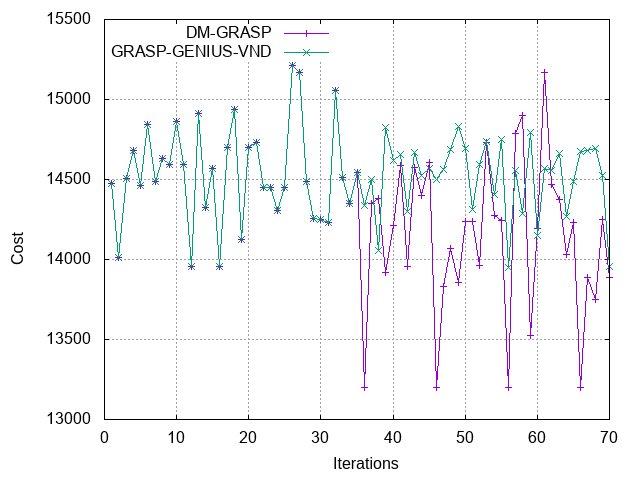
\includegraphics[width=0.8\textwidth]{construcao_grasp_dm-grasp.png}%
\caption{Construction phase}
\label{fig:cdm}
\end{figure}


\begin{figure}[!h]
	\centering
	
	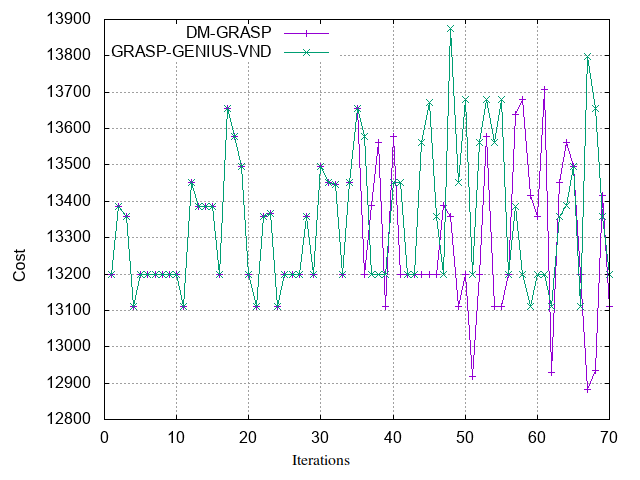
\includegraphics[width=0.8\textwidth]{buscalocal_grasp_dm-grasp.png}%
	\caption{Local search phase}
	\label{fig:bldm}
\end{figure}

The same analysis with DM-GRASP on the impact of using mined patterns was also carried out with MDM-GRASP. From Figures \ref{fig:cmdm} and \ref{fig:blmdm}, it can be observed that after the MD process, the construction and local search phases present similar lines for the two data mining strategies, demonstrating, in this way, similar behaviours. For the instance used in the experiment, MDM-GRASP performed the data mining procedure four times, after iterations 10, 34, 48, and 62. Unlike DM-GRASP, it is possible to verify that MDM-GRASP, after the first run of mining, continues to slightly and gradually reduce the cost of solutions obtained by construction, as patterns are extracted more than once.

It is also observed that the proposed strategies are able to better explore the search space. There are several situations where state-of-the-art heuristics perform this exploration inefficiently. For example, in Figure \ref{fig:blmdm}, it can be seen that the value obtained by the GRASP-GENIUS-RVND local search does not change from iterations 5 to 10, 13 to 15, 25 to 27 and 37 to 39 In the specific execution of this experiment, this behaviour tends to occur less when there is an application of MD.


\begin{figure}[!h]
	\centering
	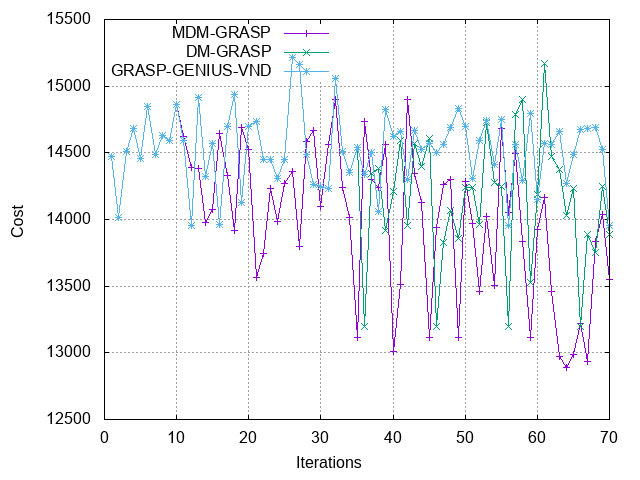
\includegraphics[width=0.7\textwidth]{construcao_mdm_dm_grasp.png}
	\caption{Construction phase}
	\label{fig:cmdm}
\end{figure}


\begin{figure}[!h]
	\centering
	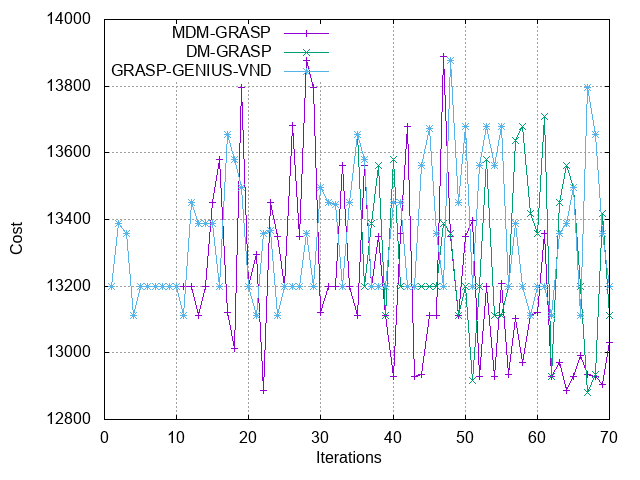
\includegraphics[width=0.7\textwidth]{buscalocal_mdm_dm_grasp.png}
	\caption{Local search phase}
	\label{fig:blmdm}
\end{figure}

In Tables \ref{tab:dm-grasp} and \ref{tab:mdm-grasp}, it was verified that the main contribution of the MD application in the state-of-the-art heuristic is in the reduction of computational time spent. Figures \ref{fig:md-tempo-c} and \ref{fig:md-tempo-bl} illustrate the behaviour of the construction and local search phases, in terms of computational time used by GRASP-GENIUS-RVND, DM -GRASP and MDM-GRASP, by running 70 iterations of instance g\_kroA150\_VT30\_T30\_W90\_50. The figures show that, for all strategies, the local search phase took more time than the construction phase. Since in the DM-GRASP strategy, the data mining process is executed after iteration 35, it can be seen in Figure \ref{fig:md-tempo-c} that, from this point onwards, the computational time spent by the construction phase is reduced. Originally, the construction of a route is started by selecting three random vertices and then vertices are inserted into the route until all the constraints of the problem are satisfied. With the application of MD, this insertion of vertices takes place from a mined pattern, which usually has more than three vertices, which reduces the number of insertions necessary to satisfy all the conditions of the problem and, consequently, reduces the computational time spent.

The GRASP-GENIUS-RVND local search is performed by the RVND heuristic. This strategy is terminated only when all types of Neighbourhoods are explored, and for each new solution improvement, RVND restarts its process from the first Neighbourhood in the list. As the solutions generated by the construction from the patterns are generally closer to an optimal location, in Figure \ref{fig:md-tempo-bl}, it can be observed that the exploration of all types of Neighbourhoods is performed more quickly, as fewer improvements are made, and RVND returns fewer times to the first Neighbourhood in the list.

In the MDM-GRASP strategy, the data mining process is performed more than once. As can be seen in Figures \ref{fig:md-tempo-c} and \ref{fig:md-tempo-bl}, MDM-GRASP behaves similarly to DM-GRASP until the moment when the first mining is carried out. From this iteration onwards, the more MD processes are executed, the computational times of the construction and local search phases are gradually and slightly reduced.

\begin{figure}[!h]
	\centering
	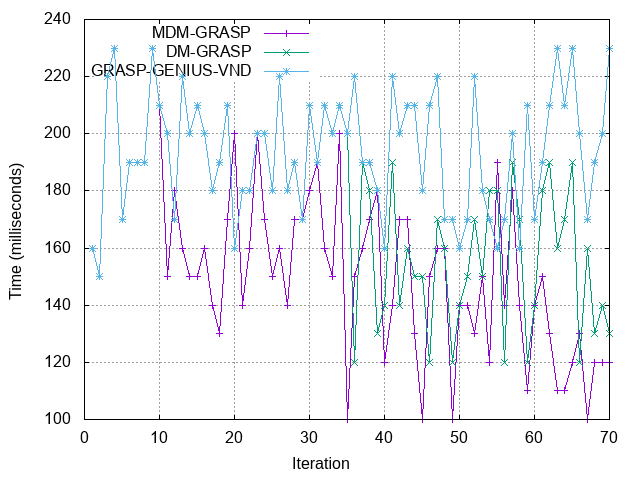
\includegraphics[width=0.7\textwidth]{md-tempo-construcao.png}
	\caption{Construction phase}
	\label{fig:md-tempo-c}
\end{figure}

\begin{figure}[!h]
	\centering
	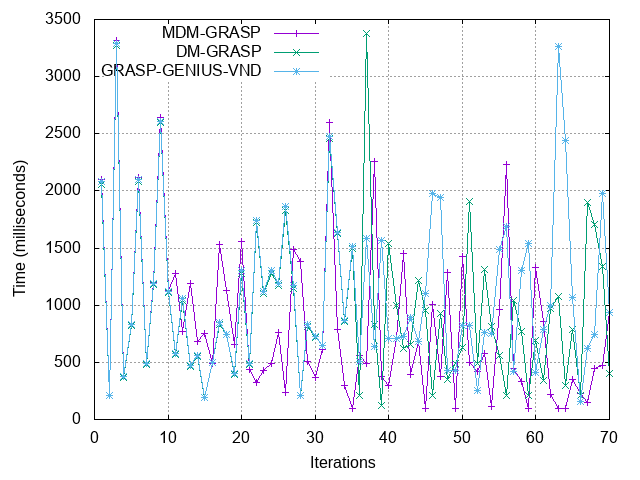
\includegraphics[width=0.7\textwidth]{md-tempo-bl.png}
	\caption{Local search phase}
	\label{fig:md-tempo-bl}
\end{figure}

\subsection{Statistical tests}

To strengthen the performance evaluation of the proposed methods, statistical significance tests (SST) were performed in all instances. Through the application of this test, the objective is to verify, in statistical terms, whether the results generated by the heuristics indicate a statistical difference, reinforcing the relevance of the application of MD and PLI, or not.


Generally, this type of test is used to evaluate algorithms that have random components, and identify whether
the difference between their means was due to the superiority of one of these algorithms or just due to the randomness present in the methods. In this work, the non-parametric statistical test of \textit{Friedman} \cite{siegal1956nonparametric} of the R package \cite{r-package} was used, which does not require that the analysed sample follow a normal distribution.

To perform this test, the costs obtained for ten executions of each heuristic were considered, $p$-value equal to 0.05 and two hypotheses:

\begin{itemize}
\item Null Hypothesis ($H_0$): There is no difference between the means found by the two methods; and

\item Alternative hypothesis ($H_1$): There is a difference between the means found by the two methods.
\end{itemize}


In this sense, $H_0$ will be rejected with 95\% certainty if, for each instance, the test of \textit{Friedman} \cite{siegal1956nonparametric} returns a value less than the defined $p$-value.
If $H_0$ is rejected, the alternative hypothesis $H_1$ is considered.

In Table \ref{tab:sig1}, for each pair of compared heuristics, the number of wins, losses and ties in terms of best solution, average solution and average time spent is shown. For the solution mean, the values in parentheses indicate the number of statistically significant results. MDM-GRASP was not directly compared with the state-of-the-art heuristic, but with DM-GRASP in Table \ref{tab:mdm-grasp}. Table \ref{tab:sig1}, presents a summary of what can be deduced from Tables \ref{tab:dm-grasp} and \ref{tab:mdm-grasp}, in relation to a comparison between MDM- GRASP and GRASP-GENIUS-RVND.

\begin{table}[!h]
\centering
\caption{Summary of results and statistical significance test between GRASP-GENIUS-RVND and MDM-GRASP.}
\label{tab:sig1}
\begin{tabular}{llll}
\hline
& Best Sol. & Average Sol. & Average T(s) \\
\hline
\begin{tabular}[c]{@{}l@{}}Win\\ MDM-GRASP\end{tabular} & 13 & 41 (10)& 105 \\ \hline
Ties & 90 & 50 & 0 \\ \hline
\begin{tabular}[c]{@{}l@{}}Win\\ GRASP-GENIUS-RVND\end{tabular} & 4 & 16 (0) & 2\\
\hline
\end{tabular}
\end{table}

In terms of the best solution, MDM-GRASP was superior in 13, tied in 90 and lost in 4 instances. Regarding the average solution, the mining heuristic won in 41 cases, ten of which were statistically significant, tied in 50 and lost in 16 instances. For this statistical test, it was observed that the significant results obtained are concentrated in the larger instances, including gr202\_R39\_T122\_W41\_25, gr229\_R45\_T46\_W138\_25, lin318\_R108\_T105\_W105 \_50, rd400\_R80\_T240\_W80\_25, among others. As already noted in previous sections, the application of data mining reduces the computational time of the heuristics. With MDM-GRASP it was no different, being faster than the state-of-the-art heuristic in 105 of the 107 instances tested, and with an average CPU-time reduction of 23.55\% per instance.

\subsection{TTTPlots}

A final comparison was made between the proposed methods and the state-of-the-art, using \textit{Time-to-target plots} (\texttt{TTTplots}) \cite{aiex2007ttt}. These types of plots are used to analyse the behaviour of algorithms with random components and show the cumulative probability of an algorithm to find a solution better than or equal to a predefined target solution value, in a certain running time.

The TTTplots illustrated in Figure \ref{fig:tttplots1} were generated from 100 executions of the GRASP-GENIUS-RVND and MDM-GRASP methods using the instance g\_kroA150\_VT30\_T30\_W90\_50, and  seeds ranging from 1 to 100. For the behaviour analysis, a difficult target value was chosen, the value of the best solution reported in this instance by GRASP-GENIUS-RVND (12918).

\begin{figure}[!h]
\centering
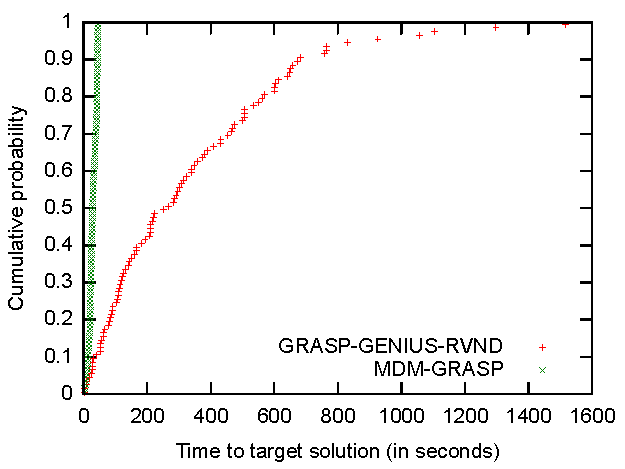
\includegraphics[width=0.7\textwidth]{tttplot.pdf}
\caption{TTTplots for instance g\_kroA150\_VT30\_T30\_W90\_50, target: 12962.}
\label{fig:tttplots1}%
\end{figure}

From Figure \ref{fig:tttplots1}, a large difference can be seen between the curves of the compared heuristics. After 561 seconds of execution, GRASP-GENIUS-RVND reaches the target with a probability of 79\%, while with that same chance, MDM-GRASP only needs 41.71 seconds to reach the target.

\section{Conclusions}

\label{sec:conclusions}

In this work, we have proposed two hybrid heuristics, DM-GRASP and MDM-GRASP, using DM techniques over a state-of-the-art heuristic (GRASP-GENIUS-RVND). These heuristics perform data mining along the iterative process of the GRASP-GENIUS-RVND and extract patterns detected in high- quality solutions, which are used to generate further initial solutions. 

As the source-code was provided by the authors, all GRASP-GENIUS-RVND experiments mentioned in \citet{daSilva} were completely re-executed in order to offer a fair and strict evaluation of the computational results. In addition, to assist the evaluation of the heuristics,  examples of the influence of mining patterns on early solutions, analyses of time convergence (TTTplots), and statistical significance tests were performed.

The reported results demonstrated that both DM strategies perform better than the state-of-the-art heuristic, in terms of solution quality and CPU time simultaneously. Both DM-GRASP and MDM-GRASP heuristics managed to apply a significant reduction in execution time, confirming the various reports in the literature on the application of such techniques. MDM-GRASP, for example, which was the heuristic with the best performance among the three compared, was able to reduce the GRASP-GENIUS-RVND time by 88.1\% for the instance pr226\_R44\_T46\_W136\_75.

As a further investigation, we intend to combine the MDM-GRASP with integer programming techniques. Since it was observed that mined patterns can help in the construction of initial solutions, we see the possibility of applying them to the exact resolution of an IP model through branch-and-bound, on fixing variables, providing a ``warm start'', or guiding the variable selection for branching.


%\bibliographystyle{model1-num-names}
\bibliographystyle{apalike}

% Loading bibliography database
\bibliography{cas-refs}


\end{document}

